%-------------------------------------------------------------------------------
% This file provides a skeleton ATLAS note.
\pdfinclusioncopyfonts=1
% This command may be needed in order to get \ell in PDF plots to appear. Found in
% https://tex.stackexchange.com/questions/322010/pdflatex-glyph-undefined-symbols-disappear-from-included-pdf
%-------------------------------------------------------------------------------
% Specify where ATLAS LaTeX style files can be found.
\RequirePackage{latex/atlaslatexpath}
% You can comment out the above line if the files are in a central location, e.g. $HOME/texmf.
%-------------------------------------------------------------------------------
\documentclass[NOTE, REPORT=false, atlasdraft=true, UKenglish]{atlasdoc}
% The language of the document must be set: usually UKenglish or USenglish.
% british and american also work!
% Commonly used options:
%  atlasdraft=true|false This document is an ATLAS draft.
%  texlive=YYYY          Specify TeX Live version (2020 is default).
%  NOTE                  The document is an ATLAS note (draft).
%  REPORT=true|false     Use scrreprt|scrartcl as main class for document.
%  txfonts=true|false    Use txfonts rather than the default newtx.
%  paper=a4|letter       Set paper size to A4 (default) or letter.

%-------------------------------------------------------------------------------
% Extra packages:
\usepackage[subcaption]{atlaspackage}
% Commonly used options:
%  backend=bibtex        Use the bibtex backend rather than biber.
%  subfigure|subfig|subcaption  to use one of these packages for figures in figures.
%  minimal               Minimal set of packages.
%  default               Standard set of packages.
%  full                  Full set of packages.
%-------------------------------------------------------------------------------
% Style file with biblatex options for ATLAS documents.
\usepackage{atlasbiblatex}
% Commonly used options:
%  backref=true|false    Turn on or off back references in the bibliography.

% Package for creating list of authors and contributors to the analysis.
\usepackage{atlascontribute}

% Useful macros
\usepackage{atlasphysics}
% See doc/atlas_physics.pdf for a list of the defined symbols.
% Default options are:
%   true:  journal, misc, particle, unit, xref
%   false: BSM, hepparticle, hepprocess, hion, jetetmiss, math, process,
%          other, snippets, texmf
% See the package for details on the options.

% Macro to add to-do notes (for several authors). Uses the todonotes package.
% \ATLnote{JS}{Jane}{green!20}{green!50!black!60}
% add macros \JSnote and \JSinote for notes in the margin and inline.
% The first colour is for the body and the second for the border of the note.
% Set output=false in order not to print out the notes.
% Set shift=false to avoid adjustment of margins.
% Check for notes still left by commenting out the package in the final version of the note.
\usepackage[output=true, shift=true]{atlastodo}
\usepackage{comment} 

%TODO notes, author notes deinitions
\ATLnote{AS}{Alex}{cyan!20}{cyan}

% Files with references for use with biblatex.
% Note that biber gives an error if it finds empty bib files.
\addbibresource{ANA-HIGP-2024-02-INT1.bib}
\addbibresource{bib/ATLAS.bib}
\addbibresource{bib/CMS.bib}
\addbibresource{bib/ConfNotes.bib}
\addbibresource{bib/ATLAS-useful.bib}
\addbibresource{bib/PubNotes.bib}


% Paths for figures - do not forget the / at the end of the directory name.
\graphicspath{{logos/}{figures/}}

% Add your own definitions here (file ANA-HIGP-2024-02-INT1-defs.sty).
\usepackage{ANA-HIGP-2024-02-INT1-defs}

%-------------------------------------------------------------------------------
% Generic document information.
%-------------------------------------------------------------------------------

% Title, abstract and document.
%-------------------------------------------------------------------------------
% This file contains the title, author and abstract.
% It also contains all relevant document numbers used for an ATLAS note.
%-------------------------------------------------------------------------------

% Title
\AtlasTitle{Measurement of fiducial and differential cross sections in the $H\rightarrow\gamma\gamma$ decay channel with 168 $\text{fb}^{-1}$ of 13.6 $\text{TeV}$ proton–proton collision data with the ATLAS detector}

% Draft version:
% Should be 1.0 for the first circulation, and 2.0 for the second circulation.
% If given, adds draft version on front page, a 'DRAFT' box on top of each other page, 
% and line numbers.
% Comment or remove in final version.
\AtlasVersion{0.1}

% Abstract - % directly after { is important for correct indentation
\AtlasAbstract{%
  We present supporting documentation for fiducial and differential cross-section measurements of the Higgs boson in the $H\rightarrow\gamma\gamma$ decay channel using 168 $\text{fb}^{-1}$of proton--proton collisions recorded at 13.6 $\text{TeV}$ centre of-mass energy in the years 2022 to 2024.
  %The amount of background, mainly from SM diphoton production and hadronic jets, is determined by a simultaneous signal and background fit to the diphoton mass spectrum.
  The fiducial cross-section is measured in few inclusive phase space regions, and differentially as functions of a selection of variables.
  %The data is compared to several state-of-the-art theoretical predictions of SM Higgs boson production.
}

% Author - this does not work with revtex (add it after \begin{document})
\author{The ATLAS Collaboration}

% Authors and list of contributors to the analysis
% \AtlasAuthorContributor also adds the name to the author list
% Include package latex/atlascontribute to use this
% Use authblk package if there are multiple authors, which is included by latex/atlascontribute
% \usepackage{authblk}
% Use the following 3 lines to have all institutes on one line
% \makeatletter
% \renewcommand\AB@affilsepx{, \protect\Affilfont}
% \makeatother
% \renewcommand\Authands{, } % avoid ``. and'' for last author
% \renewcommand\Affilfont{\itshape\small} % affiliation formatting
\AtlasAuthorContributor{HUSTON, Joey}{a}{Product-cut studies}
\AtlasAuthorContributor{JIN, Shan}{b}{ }
\AtlasAuthorContributor{MIJOVIC, Liza}{c}{Analysis contact, Signal modelling, Asimov fits}
\AtlasAuthorContributor{MARTIN, Victoria}{c}{Supervisor/PI of Julia Allen, Alex Sopio.}
\AtlasAuthorContributor{TURRA, Ruggero}{d}{ }
\AtlasAuthorContributor{MANZONI, Stefano}{e}{ }
\AtlasAuthorContributor{CUETO GOMEZ, Ana Rosario}{f}{Variable selection \& binning optimisation.}
\AtlasAuthorContributor{TAREK, Ahmed}{e}{ }
\AtlasAuthorContributor{D'ERAMO, Louis}{h}{ }
\AtlasAuthorContributor{MUNGO, Davide}{i}{ }
\AtlasAuthorContributor{XIA, Ligang}{b}{ }
\AtlasAuthorContributor{PASCUAL DOMINGUEZ, Luis}{f}{Analysis contact}
\AtlasAuthorContributor{SOPIO, Alex}{c}{INT Note editor, 2x2D background estimation.}
\AtlasAuthorContributor{NASELLA, Laura}{d}{ }
\AtlasAuthorContributor{KAFLE, Pratik}{a}{Product-cut studies}
\AtlasAuthorContributor{ALLEN, Julia Frances}{c}{Signal modelling, mc21 vs. mc23 cross-checks.}
\AtlasAuthorContributor{ZHOU, Yong}{b}{INT Note editor, spurious signal.}
\AtlasAuthorContributor{COLLADO SOTO, Pablo}{f}{ }

%\AtlasContributor{Fourth AtlasContributor}{b}{Contribution to the analysis.}
%\author[a]{First Author}
% \author[a]{Second Author}
% \author[b]{Third Author}
\affil[a]{Michigan State University}
\affil[b]{Nanjing University}
\affil[c]{University of Edinburgh}
\affil[d]{Università degli Studi di Milano}
\affil[e]{CERN}
\affil[f]{Universidad de Madrid}
\affil[h]{Université Clermont Auvergne}
\affil[i]{University of Toronto}


% If a special author list should be indicated via a link use the following code:
% Include the two lines below if you do not use atlasstyle:
% \usepackage[marginal,hang]{footmisc}
% \setlength{\footnotemargin}{0.5em}
% Use the following lines in all cases:
% \usepackage{authblk}
% \author{The ATLAS Collaboration%
% \thanks{The full author list can be found at:\newline
%   \url{https://atlas.web.cern.ch/Atlas/PUBNOTES/ATL-PHYS-PUB-2016-007/authorlist.pdf}}
% }

% ATLAS reference code, to help ATLAS members to locate the paper
\AtlasRefCode{ANA-HIGP-2024-02}

% ATLAS note number. Can be an COM, INT, PUB or CONF note
\AtlasNote{ANA-HIGP-2024-02-INT1}

% Author and title for the PDF file.
\hypersetup{pdftitle={ATLAS document},pdfauthor={The ATLAS Collaboration}}

%-------------------------------------------------------------------------------
% Content
%-------------------------------------------------------------------------------
\begin{document}

\maketitle
\PrintAtlasContribute{0.35}
\clearpage

% List of to-do notes.
% \listoftodos

\section*{Changelog and To-do list}
\subsection*{Changelog}
\begin{itemize}
    \item v0.1: First version of doc for CDS.
    \item v0.2: Updated version. Filling in sections to document work done to-date.
    \begin{itemize}
        \item \textbf{Introduction} provided more specific context for the Run 3 analysis. 

        \item \textbf{Section 3 Object Definitions and Event Selection}: added up-to-date Run3 object descriptions and their references.
        
        \item \textbf{Section 5 Signal and Background modelling}: replaced initial spurious signal studies with a much more advanced study, including proper background decomposition, GPR smoothing and low-stats categories treatment
        
        \item \textbf{Section 6 Background Estimation}: added results for all differential categories.
        
        \item \textbf{Section 7 Uncertainties}: added descriptions of experimental uncertainties. Theoretical uncertainties are still to be evaluated.
        
        \item \textbf{Section 9 Signal Yield Extraction}: added more detailed descriptions to improve clarity.
        
        \item \textbf{Section 12 Conclusion} added a preliminary conclusion paragraph, to be updated once results are finalised.
        
        \item \textbf{New appendices}: Background Templates, Data Sidebands for Wald tests, Truth Isolation Studies. 
    \end{itemize}
\end{itemize}

\section*{Publication timeline}

\begin{table}[h]
    \centering
    \begin{tabular}{|l|l|}
        \hline
        \textbf{Date} & \textbf{Event}  \\
        \hline
        2025/08/05 & EB request \\
        2025/10/24 & All studies to-date updated in INT note \\
        2026/02 & Publication target (Moriond) \\
        \hline
    \end{tabular}
    \caption{Analysis timeline, as of October 2025.}
\end{table}


%\listoftodos
\section*{To-do list (Status October 2025)}

Main analysis TO-DO items: 
 \begin{itemize}
    \item Cross-checks with new product cuts; if successful, product cuts will
    be adopted for the analysis

    \item Theoretical uncertainties 

    \item Implement fix for timing-cut in isolation calculation. Recompute background.
\end{itemize}
Other TO-DO items:
    \begin{itemize}
    \item Unfolding using matrix-inversion instead of bin-by-bin correction factors.

    \item Full systematic uncertainties to replace simplified scheme.

    \item Analysis CP task, currently $\sim$ 1/3 complete (\href{https://its.cern.ch/jira/browse/ATLASEG-426}{link to JIRA ticket}).
 
\end{itemize}



 
\clearpage


\tableofcontents

%-------------------------------------------------------------------------------
%-------------------------------------------------------------------------------
% You can find some text snippets that can be used in papers in \texttt{latex/atlassnippets.sty}.
% To use them, provide the \texttt{snippets} option to \texttt{atlasphysics}.


\section{Introduction}
\label{sec:introduction}
This note presents the measurement of the total and differential cross-sections
of Higgs Boson decays to two photons ($H \to \gamma \gamma$) in $168
\,\mathrm{fb}^{-1}$ of proton-proton collision data, collected at a
center-of-mass energy of $13.6\,\mathrm{TeV}$ with the ATLAS detector at the
Large Hadron Collider (LHC). The measurement follows previous analyses by ATLAS
at $8 \,\mathrm{TeV}$~\cite{HIGG-2013-10}, $13
\,\mathrm{TeV}$~\cite{HIGG-2022-04} and $13.6 \,\mathrm{TeV}$ in combination
with $H \to ZZ$~\cite{HIGG-2022-12}. This analysis follows closely the strategy
employed in the early Run 3 ATLAS measurements using $31.4\, \mathrm{fb}^{-1}$
at $13.6\,\mathrm{TeV}$, and Run 2 analysis using $140 \,\mathrm{fb}^{-1}$ at
$13\,\mathrm{TeV}$. Significant changes made in this analysis include using
updated CP recommendations and modifications to set of the studied variables.
Potential further change under consideration is a switch to to so-called
product di-photon cuts for the event selection. 

This section introduces the measurement, motivates its significance, and presents an overview of the analysis strategy. 

\subsection{Motivation}

During Run 3 of the LHC, the ATLAS experiment collected its largest dataset so far and at a new, higher, proton-proton collision energy of $13.6\,\mathrm{TeV}$. This dataset provides a unique opportunity for precision measurements of the Higgs boson’s properties, including in the $H \to \gamma \gamma$ decay channel, where the Higgs boson signal is well-resolved due to its narrow resonance mass.

However, there is a large background to the $\gamma\gamma$ final state due to production of two high-energy photons which are not produced from Higgs boson decay.  
The size and shape of this background is hard to predict, but should not peak around the Higgs mass.  The analysis presented in this note relies on a data-driven technique to model the background.

The fiducial cross section of a scattering process is a measurement of the cross section in a defined volume of phase space, typically one that can be easily and consistently defined in an experimental and theoretical context, and therefore can be used to make a comparison between observations and theoretical predictions. 
In this note, we define the \textit{inclusive fiducial volume} a volume of phase space similar to the acceptance of the ATLAS detector.

The inclusive fiducial volume is defined as the region to observe two isolated photons in the pseudorapidity range $|\eta|<1.37$ or $1.52<|\eta|<2.37$ and the photon transverse momentum satisfying $\ptgg > 0.35 (0.25)$; where $\ptgg{}$ is the invariant mass of the two photons. 

Differential cross section measurements looks at the how the production of the Higgs boson varies in different regions of phase space, e.g.~as a function of different kinematic variables with additional particles in the final state.   These distributions are sensitive to the properties of the Higgs boson, including its mass and couplings.  
%The Higgs boson is the most recently discovered fundamental particle, its properties, including couplings, are still not fully characterised.  
If the Higgs boson couples to BSM particles this might first become apparent in the tails of fiducial cross section measurements.

By comparing the rate and shape of the differential cross sections with theoretical predictions, we can look for any deviations; deviations could be a sign of new physics, or they could indicate a limitation or poor choice of parameters in the model we are comparing to.
In this note we look at the fiducial cross section for $pp \to H \to \gamma \gamma$ production using variables sensitive to different production mechanisms and couplings.

%% more detail to be added here about specific cuts 


\subsection{Differential Variables}

The differential cross section is measured using several different variables: 
the choice of which variables to use for the differential cross section are motivated by the predicted significance of the distributions, from considerations of the different production mechanisms and with an aim to characterise the production as fully as possible given the data set.

The variables are described in detail in section~\ref{sec:differentialobservables}.  They include kinematic properties of the photon-pair, the numbers of jets and charged leptons produced in association, and kinematic properties of any jet pairs.  The binning of the variables is chosen to optimise significance, to minimisation corrections apply at unfolding and to facilitate combination with other analyses. 


%%% TODO: A detailed motivation of the measurement should go here
% - The Run 2 INT note should be a good template https://cds.cern.ch/record/2714980/files/ATL-COM-PHYS-2020-253.pdf 
% - State the purpose of the measurement and provide some theoretical context 
% - Give a very brief description of the measurement
% - Describe fiducial sub-regions
% - Give a description of the kinematic variables for which we have studied the differential XSections

\subsection{Analysis Strategy}
The strategy used in this analysis is similar to previous analyses~\cite{HIGG-2013-10, HIGG-2022-04, HIGG-2022-12} and is summarised briefly here:
\begin{itemize}
\item The data and simulated samples used are presented in Section~\ref{sec:samples};

\item Events are selected for further analysis, the selection criteria follows closely the definition of the fiducial region; 
the definition of the physics objects and event selection criteria is described in Sections~\ref{sec:EventSelections} and~\ref{sec:fiducial}.

\item Differential cross sections are defined  by dividing the inclusive cross section volume into several exclusive bins.  The choice of variables and binning is presented in Section~\ref{sec:observablesbinning};

\item Section~\ref{sec:signalbackgroundmodelling} discusses the modelling of the background and signal as a function of the di-photon invariant mass $\mgg{}$;
analytical fits are made to understand the background in each fiducial cross section bin and in the inclusive fiducial cross section.



\item  The residual background, including potential spurious signal is estimated.  The main sources of background are non-resonant production of diphotons and events where hadronic jets are misreconstructed as photons.  To estimate the background  the  \twoxtwod\ method is used; double two-dimentional sidebands are defined using using $\mgg{}$ and changing the selection criteria used to select photons.  This is presented in Section~\ref{sec:backgroundestimation}.

\item  Uncertainties due to systematic effects and theoretical modelling are explored and quantified in Section~\ref{sec:uncertainties}.

\item The fiducial cross sections in terms of observed variables is highly
  dependent on the experimental setup (detector effects); in order to present
  results independent of the experiment, the cross sections are
  \textit{unfolded} to remove detector effects.  The unfolding procedure is
  presented in Section~\ref{sec:unfolding}.

\item The cross section for the signal is extracted by fitting the observed $\mgg{}$ distribution to the signal and background as described in Section~\ref{sec:signalyieldextraction}.
  
\item Section~\ref{sec:asimovresults} presents the expected results; the observed results and conclusions are presented in Sections~\ref{sec:dataresults} and~\ref{sec:conclusion}.

\end{itemize}

\section{Data and simulation samples}
\label{S. Data and MC Samples}
The analysis is performed on data and simulation samples reconstructed with
Athena release 23.
The input are HIGG1D1 derivations produced with AthDerivation cache 25.0.22;
the corresponding p-tags are p6456 (data), p6599 (signal MC), p6453/p6781 (background MC).
The full list of input DAODs is given in appendix~\ref{app:DAODs}.

The HIGG1D1 derivation applies a looser preselection than the one applied
offline.
In particular, events are required to pass the logical OR of various diphoton
triggers and to contain at least two offline photon candidates.

All samples are then analysed with the HGamCore analysis framework~\cite{HGamCore}.
Mini xAODs (MxAODs) are produced by the HGamma group and stored in /eos.
The 'h032' tag was used for the MxAOD production, on top
of AnalysisBase 25.2.43.
At this stage all particle candidates are calibrated, data and simulation
corrections and weights are computed and applied or saved in the MxAOD,
and a few extra variables useful for the analysis are calculated.
A preselection is performed, that requires the following:
\begin{itemize}
\item Duplicate events are removed
\item Data events must pass the good runs lists requirement (good data quality)
\item Events must be collected with at least one of several diphoton triggers
  (including the one used by this analysis).
\item Data events must pass detector quality flags.
  Events with data integrity errors in the calorimeters and
  incomplete events where some detector information is missing are rejected.
\item The event must have at least one primary vertex candidate
\item There must be at least two photon candidates passing loose identification
  requirements based on their shower shapes in the electromagnetic calorimeter
  and the leakage in the hadronic calorimeter, and not passing through
  regions of the calorimeter with cells connected to dead high-voltage lines.
\end{itemize}

Special MxAODs (``DetailedNoSkim'') without any selection applied
are produced for the signal MC samples that are used to compute
the response matrices needed for the unfolding.

The MxAODs are a single format common to several Higgs to diphoton analyses,
such as the measurement of Higgs boson couplings and simplified template
cross sections, search for Higgs bosons produced in association with dark
matter and so on.
For this reason they are rather large, containing many more variables (several
hundreds) than needed for this analysis.
For this reason, MxAODs are further skimmed into micro-xAODs (uxAODs) of
smaller size, with only the needed variables (at detector and particle level)
and only the events of interest (typically, the full selection is applied for
data and background MC uxAODs, while for signal MC uxAODs events that pass
the full selection or are in the fiducial volume are kept).

\subsection{Data samples}
\label{ssec:samples:data}
This analysis is based on partial run3 $pp$ collision data collected by ATLAS detector at central-of-mass energy $\sqrt{s}$ = 13.6 TeV between 2022 and 2024.After data quality requirements are applied to ensure that all the detector components are in good working condition The total corresponding integrated luminosity is 168 \ifb.The corresponding GRLs for each year are summarized in Table~\ref{tab:lumi_grl}.

Events are selected if thet pass either a diphoton trigger or single photon trigger\cite{egamma_trigger}.The diptoton trigger has a transverse energy thresholds of 35GeV and 25GeV for the leading and subleading photon candicates respectively,with medium photon identification based on calorimeter shower shape variables.The single-photon photon trigger require the transverse enegry of the leading photon greater than 140 GeV and pass the loose photon identification.On average,the trigger efficiency is greater than 98\% for the events pass the diphoton event selection.However,The additional improvement from the single photon trigger is less than 1\% . Table ~\ref{tab:trig} summarized the HLT diphoton trigger for each year. 

\begin{table}[!htbp]
  \centering
  \scriptsize
  \begin{tabular}{clc}
    %\hline\hline
    \toprule
    Year & GRL & Luminosity (\ifb) \\
    \hline
    2022 & \texttt{\tiny data22\_13p6TeV.periodAllYear\_DetStatus-v109-pro28-04\_MERGED\_PHYS\_StandardGRL\_All\_Good\_25ns\_ignore\_TRIGMUO\_TRIGLAR.xml} & 31.39 \\
   %\hline
    2023 & \texttt{\tiny data23\_13p6TeV.periodAllYear\_DetStatus-v110-pro31-06\_MERGED\_PHYS\_StandardGRL\_All\_Good\_25ns\_ignoreTRIG\_JETCTPIN.xml}  & 27.23\\
    %\hline
    2024  & \texttt{\tiny physics\_25ns\_data24.xml} & 109.4\\
    \hline
    Total  & -  & 168\\    
    \bottomrule
  \end{tabular}
  \caption{The corresponding GRL and luminosity for each year}
  \label{tab:lumi_grl}
\end{table} 

\begin{table}[htbp]
    \centering
    \begin{tabular}{c|c}
      \toprule
        Year & trigger \\
        \hline
        2022 & \texttt{HLT\_g35\_medium\_g25\_medium\_L12EM20VH} \\
        \hline
        2023 & \texttt{HLT\_g35\_medium\_g25\_medium\_L12eEM24L} \\
        \hline
        2024 & \texttt{HLT\_g35\_medium\_g25\_medium\_L12eEM24L} \\
        \bottomrule
    \end{tabular}
    \caption{The di-photon trigger used by this analysis for each year.}
    \label{tab:trig}
\end{table}

\subsection{Simulation samples}
\label{ssec:samples:mc}

Simulated event samples are used to estimate the expected signal yield,
to optimize the binning of the differential cross section measurements,
to model the signal diphoton invariant mass for the fit to the data used to
determine the signal and background yields,and to estimate the correction factors to unfold the detector-level yields to the particle-level ones.
They are also used to determine the relative fractions of different
type of backgrounds and build, with the help of data control regions,
a background-only template that is used to choose an analytic function
to model the diphoton invariant mass distribution of the background and to
estimate the corresponding systematic uncertainty on the signal yield
determined from the signal+background fit to the data.

The event generators used to generate the nominal signal and background events,
the PDFs used for the matrix element generation, and the number of generated
events are summarized in Table~\ref{tab:samples:nominal_mc}.
The generated signal events were then passed to the full ATLAS detector
simulation based on Geant 4, while generated QCD diphoton events were passed
through a fast simulation of the ATLAS detector to reduce the amount of CPU
needed given the large numbers of events generated.

The matrix element for the nominal signal samples are generated with \POWHEGBOX[v2]~\cite{Nason:2009ai,Alioli:2010xd,Nason:2004rx,Frixione:2007vw}.The simulation achieved NNLO accuracy for arbitrary inclusive \(gg\to H\) observables by reweighting the Higgs boson rapidity spectrum in \textsc{Hj}-\MINLO~\cite{Hamilton:2012np,Campbell:2012am,Hamilton:2012rf} to that of HNNLO~\cite{Catani:2007vq}.The VBF, $t\bar{t}H$ and $b\bar{b}H$ processes were simulated at next-to-leading-order (NLO) accuracy in QCD.The WH and ZH were simulated by following the \MINLO~\cite{Hamilton:2012np} approach,while the ggZH was only computed at leading order(LO) in QCD.

All the signal sample matrix element use the PDFLHC21 PDF set and the generated events are showered with Pythia8 parton shower with A14 tune in which the $H \to \gamma\gamma $ is simulated.In contrast to full Run2 sample.The Dalitz decay of $H \to \gamma\gamma^* \to \gamma ff$ is not considered in the generation, where $\gamma^*$ is an off-shell photon and $f$ is any charged fermion.
% Samples of simulated $tH$ events are also available; however, we estimated
% the contribution of this production mode to the analysis to be negligible
% and therefore they won't be used in the final analysis results (they are
% listed here for completeness).

The continuum diphoton background samples are generated with Sherpa 2.2.14.in this set-up, NLO-accurate matrix elements for up to one parton, and LO-accurate matrix elements for up to three partons were calculated with the Comix~\cite{Gleisberg:2008fv} and
\OPENLOOPS~\cite{Buccioni:2019sur,Cascioli:2011va,Denner:2016kdg} libraries. They were matched with the \SHERPA parton shower~\cite{Schumann:2007mg} using the \MEPSatNLO prescription~\cite{Hoeche:2011fd,Hoeche:2012yf,Catani:2001cc,Hoeche:2009rj}
with a dynamic merging cut~\cite{Siegert:2016bre} of \qty{10}{\GeV}.
Photons were required to be isolated according to a smooth-cone isolation
criterion~\cite{Frixione:1998jh}. Samples were generated using the
\NNPDF[3.0nnlo] PDF set~\cite{Ball:2014uwa}, along with the dedicated set of tuned
parton-shower parameters developed by the \SHERPA authors.


\begin{table}[!htbp]
  \centering
  \caption{Nominal simulated signal and background event samples}
  \label{tab:samples:nominal_mc}
\resizebox{\textwidth}{!}{    
  \begin{tabular}{lccccrrr}
    %\hline
    %\hline
    \toprule
    Process & DSID & Generator (ME+PS) & PDF (ME) & PDF+Tune & \multicolumn{3}{c}{Events} \\
            &      &                   &          &          & MC23a & MC23d & MC23e \\
    %\hline
    \midrule
    ggF              & 602421 & Powheg NNLOPS + Pythia & PDF4LHC21 & A14NNPDF23LO & 4.46M  & 4.46M  & 11.45M  \\
    VBF              & 601482 & Powheg+Pythia          & PDF4LHC21 & A14NNPDF23LO & 2.19M  & 2.19M  & 5.45M  \\
    $W^+H$           & 601484 & Powheg MINLO+Pythia    & PDF4LHC21 & A14NNPDF23LO & 0.30M & 0.30M & 0.61M \\
    $W^-H$           & 601483 & Powheg MINLO+Pythia    & PDF4LHC21 & A14NNPDF23LO & 0.29M & 0.30M & 0.60M \\ 
    $q\bar{q}\to ZH$ & 601523 & Powheg MINLO+Pythia    & PDF4LHC21 & A14NNPDF23LO & 0.59M & 0.59M & 1.25M \\
    $gg\to ZH$       & 601522 & Powheg+Pythia          & PDF4LHC21 & A14NNPDF23LO &   0.1M &   0.1M &   0.2M \\
    $t\bar{t}H$      & 602422 & Powheg+Pythia          & PDF4LHC21 & A14NNPDF23LO & 0.79  & 0.78M  & 1.98M  \\
    $b\bar{b}H$      & 601710 & Powheg+Pythia          & PDF4LHC21 & A14NNPDF23LO & 0.20M & 0.20M & 0.5M \\
    %$tHjb$           & 545636 & MG5\_aMC@NLO+Pythia   & PDF4LHC21 & A14NNPDF23LO & 0.49M & 0.46M & 1.69M \\
    %$tWH$            & 545639 & MG5\_aMC@NLO+Pythia   & PDF4LHC21 & A14NNPDF23LO &  0.49M & 0.49M & 1.74M \\
    \hline
    $\gamma\gamma$+jets, $m_{\gamma\gamma} \in$ 90--175~GeV & 700980 & Sherpa (ME@NLO+PS) & NNPDF3.0NNLO & Sherpa & 227M & 215M & 703M \\
    %\hline
    %\hline
    \bottomrule
  \end{tabular}
}
\end{table} 






Alternative signal samples were also generated in order to estimate
uncertainties related to the modelling of the parton shower or of
the matrix element and in particular of extra jet radiation in gluon fusion.
For the estimation of the uncertainties related to the modelling of
the parton shower, for the ggF, VBF, $VH$, $tH$ ($ttH$) samples the
same events from the matrix-element generator of the nominal signal
samples were showered with Herwig 7.2.3 instead of Pythia
(see Table~\ref{tab:samples:herwig_mc}),using the H7UE set
of tuned parameters~\cite{Bellm:2015jjp} and the \MMHT[lo] PDF set~\cite{Harland-Lang:2014zoa}.


%%Due to some technical issues, the VBF sample only includes the nominal
%%event weight, calculated with the NNPDF3.0 NLO (CHECK) PDF.
%For the estimation of the uncertainties related to the matrix
%element calculation, alternative samples were produced with MadGraph5
%interfaced to Pythia8 (see Table~\ref{tab:samples:mg5_mc}).
% $VH$ samples were also produced, but they only contain leptonic
% decays of the $V$ boson and are therefore not usable. The reason is
% that the MadGraph5 VBF sample was supposed to include also $VH$
% events with hadronic $V$ boson decays, but due to some mistake in
% the configuration of the central production of those samples, this
% part is missing from the VBF sample.

\begin{table}[!htbp]
  \centering
  \caption{Alternative simulated signal samples showered with Herwig 7.}
  \label{tab:samples:herwig_mc}
\resizebox{\textwidth}{!}{    
  \begin{tabular}{lccccrrr}
    \toprule
    Process & DSID & Generator (ME+PS) & PDF (ME) & PDF+Tune & \multicolumn{3}{c}{Events} \\
            &      &                   &          &          & MC23a & MC23d & MC23e \\
    \midrule
    ggF              & 604315 & Powheg NNLOPS + Herwig & PDF4LHC21 & H7UE & 4.46M  & 4.45M  & 11.45M  \\
    VBF              & 604318 & Powheg+Herwig          & PDF4LHC21 & H7UE & 2.2M  & 2.19M  & 5.45M  \\
    $W^+H$           & 604312 & Powheg MINLO+Herwig    & PDF4LHC21 & H7UE & 0.29M & 0.30M & 0.61M \\
    $W^-H$           & 604311 & Powheg MINLO+Herwig    & PDF4LHC21 & H7UE & 0.29M & 0.30M & 0.60M \\ 
    $q\bar{q}\to ZH$ & 604313 & Powheg MINLO+Herwig    & PDF4LHC21 & H7UE & 0.59M & 0.59M & 1.23M \\
    $gg\to ZH$       & 604316 & Powheg+Herwig          & PDF4LHC21 & H7UE &   0.1M &   0.1M &   0.2M \\
    $t\bar{t}H$      & 604317 & Powheg+Herwig          & PDF4LHC21 & H7UE & 0.79  & 0.78M  & 1.97M  \\
    $b\bar{b}H$      & 604314 & Powheg+Herwig          & PDF4LHC21 & H7UE & 0.20M & 0.20M & 0.5M \\
    %$tHjb$           & 545636 & MG5\_aMC@NLO+Herwig   & PDF4LHC21 & H7UE & 0.49M & 0.46M & 1.69M \\
    %$tWH$            & 545639 & MG5\_aMC@NLO+Herwig   & PDF4LHC21 & H7UE &  0.49M & 0.49M & 1.74M \\
    \bottomrule
  \end{tabular}
}
\end{table}


In all generated signal samples (nominal and alternative) the Higgs
boson mass is assumed to be 125.0~GeV and its natural width is
set to $\Gamma_H = 4.07$~MeV.

The effect of multiple interactions in the same and neighbouring bunch crossings (\pileup) was modelled by overlaying~\cite{SIMU-2020-01} the simulated hard-scattering event with inelastic proton--proton (\(pp\)) events generated from a mix of  \EPOS[2.0.1.4]~\cite{Werner:2005jf} and \PYTHIA[8.310]~\cite{Bierlich:2022pfr}.
The \EPOS events were generated with the \EPOS LHC tune~\cite{Pierog:2013ria} 
and the \PYTHIA events with the A3 tune~\cite{ATL-PHYS-PUB-2016-017} 
and the \NNPDF[2.3lo]~\cite{Ball:2012cx} set of parton distribution functions (PDF).
\PYTHIA pileup events include either a high transverse momentum (\pt) jet, 
a prompt photon, or a lepton from a $b$-hadron decay, while \EPOS was filtered to simulate all remaining pileup events in the overlay sample.The individual simulations were first reweighted to ensure a smooth connection across jet \pt then
the combination reweighted to match the distribution of the actual number of interactions per bunch crossing (\(\mu\)) measured in data.

Event weights are applied to the simulation to account for data/MC
efficiency scale factors different from one, as determined from
control samples of various particles.
Energies and momentum corrections and smearing are applied
so that the momentum scales and resolution in the simulation
agree with those in data.
The corrections provided by the various performance groups in
AnalysisBase 25.2.43. were used.

The sum of the generator-level event weights of all generated events,
the luminosity of the data to be matched and the Higgs production
cross sections and branching ratio to diphotons are used to determine
the normalization factor for each simulated signal sample.




\begin{table}[!htbp]
  \centering
  \caption{SM predictions for the Higgs boson production cross section times diphoton branching ratio.}
  \label{tab:samples:signal_xsecbr}
  \scriptsize
  \begin{tabular}{lrll}
    %\hline
    %\hline
    \toprule
    Production mode & $\sigma\times BR$ [fb] & accuracy (of $\sigma$) & total events produced in 139~\ifb \\
    %\hline
    \midrule
    ggF              & 118.4259 & N3LO(QCD), NLO(EW)         & 19896 \\
    VBF              & 9.25025  & approx NNLO(QCD), NLO (EW) &  1554 \\
    $W^+H$           & 2.01349  & NNLO(QCD), NLO(EW)         &   338 \\
    $W^-H$           & 1.285728  & NNLO(QCD), NLO(EW)        &   216 \\
    $q\bar{q}\to ZH$ & 1.830301 & NNLO(QCD), NLO(EW)         &   307 \\
    $gg \to ZH$      & 0.308493 & NLO(QCD), NLO(EW)          &    52 \\
    $t\bar{t}H$      & 1.1291176 & NLO(QCD), NLO(EW)         &   190 \\
    $b\bar{b}H$      & 1.193339  & NLO(QCD), NLO(EW)         &   200 \\
    %$tHjb$          & 0.18602  & NLO(QCD)                   &    31 \\
    %$tHW$           & 0.039044 & NLO(QCD)                   &     7 \\
    % sigma*BR from https://gitlab.cern.ch/atlas-hgam-sw/HGamCore/blob/master/HGamAnalysisFramework/data/MCSamples.config#L368
    \hline
    Total            & 135.43   & -                          & 22752 \\
%%    Total w $tH$   & 135.65   & -                          & 22789 \\
    %\hline
    %\hline
    \bottomrule
  \end{tabular}
\end{table}

\FloatBarrier
\clearpage


\section{Object Definitions and Event Selections}

In this section, we provide a summary of the different object definitions and event selections. %More details are given in the common performance note~\cite{Nomidis:2718255} and in the STXS/coupling note~\cite{Berger:2764716}.

\subsection{Object Defintions}
\label{sec:objectdefinitions}

\subsubsection{Photon Reconstruction and pre-selections}
\label{sssec:photon_preselection}
Photons are reconstructed using dynamic, variable-size energy clusters in the EM calorimeter~\cite{ATL-PHYS-PUB-2017-022}. Converted photons are reconstructed from clusters associated to inner detector track(s) matched with a conversion vertex.  Photon candidates with associated super-clusters affected by dead front-end boards in the first or second sampling or by the presence high-voltage trips affecting the three samplings or that includes a masked cell in the core are considered as bad-quality photons and not considered in the analysis. Additionally, if any of the eight central strips is masked the photon candidate is not considered.
Loose photons are defined from the list of photon candidates if they satisfy the Loose identification criteria, based on shower shapes variables defined with cells of the middle and back portions of the LAr accordion calorimeter. We pre-select loose photons requiring $\pT>\SI{25}{\GeV}$ and $|\eta_{S2}|<2.37$\footnote{$\eta_{S2}$ is the $\eta$ position of the calorimetric cluster in the second sampling of the EM calorimeter.}, vetoing the transition region between $1.37 < |\eta_{S2}| < 1.52$. The \pT used for the kinematic cuts and the invariant mass computation takes into account the correction of the $\eta$ from the diphoton primary vertex position.

Photons are calibrated using the latest Run-3 calibration corrections for the energy scale and resolution detailed in~\textcolor{red}{XXX add references}. These corrections are tagged with the model~\textcolor{red}{XXX add calibration scheme}. Unless otherwise specified, the results reported in this document are obtain with this model. 
The~\textcolor{red}{XXX add syst scheme} systematics scheme which contains 70 variations for the scale and 9 for the resolution is used in this analysis.

In order to reduce the background coming from neutral mesons decaying to photon pairs and charged particles from pile-up, an isolation requirement is applied based on both calorimeter-based and track-based requirements. The \texttt{FixedCutLoose} working point is used. The requirements of this working point are specified in \Sect{\ref{ssec:event_selection}}.

During the event selection, events are required to have at least two loose photons, and the two loose photons with the highest \pT define the Higgs candidate.

\paragraph{Diphoton vertex}
\textcolor{red}{XXX modify to include the recent NN modifs}
A Neural Network (NN) is used in order to identify the correct diphoton vertex among the primary vertices reconstructed in ATLAS. The vertex with the highest score for this NN is chosen to be the primary vertex in this analysis. The NN combines information from the longitudinal segmentation of the calorimeter (“pointing”) for these two photons, the $\Delta\phi$ between the tracks of the vertices under consideration and the diphoton system, the scalar sums of tracks \pT and \pTsq. Two NN are trained, one for unconverted photons pairs and one for pairs with at least one converted photon. The neural network performs better than the usual hardest vertex requirement in identifying the truth vertex within \SI{0.3}{\milli\meter}, in particular for processes with a small number of tracks in the final state, like \ggH. 
%A comparison study of the vertex selection efficiencies for various production modes was performed in the context of the \Hyy STXS/couplings analysis~\cite{Berger:2764716}: it has been shown that the efficiency of the \ggH production modes increases from 54\% to 65\% when the NN vertex is used in place of the usual hardest one as shown in \Fig{\ref{fig:myy_vertex_resolution}}.

Once the diphoton vertex has been chosen, all the objects kinematic is recomputed and all the cuts reported in below sections are related to this diphoton vertex. The more correct choice of the primary vertex improves the \myy diphoton mass resolution by 8\% inclusively, as can be observed in \Fig{\ref{fig:myy_vertex_resolution}}. The improvement is driven by the ggH production mode, where the difference in selection efficiency between the standard hardest vertex requirement and the NN classification is the largest.
%\begin{figure}[tbp]
%	\centering
%    \includegraphics[width=0.49\linewidth]{selection/PV_mode}    
%	\includegraphics[width=0.49\linewidth]{selection/vtx_resolution}
%	\caption{(Left) NN vertex identification efficiencies compared to hardest vertex ones for the different Higgs production modes. The criteria of identification is $|z_{truth} - z_{vtx}| < \SI{0.3}{\milli\meter}$. (Right) Diphoton invariant mass distributions for the events that pass the full analysis selection described in \Sect{\ref{ssec:event_selection}} when the selected primary vertex is the nominal ATLAS vertex (``Hardest") compared to the diphoton Neural Network one.}
%	\label{fig:myy_vertex_resolution}
%\end{figure}


\subsubsection{Electron, muon, jet and \MET selections}
\textcolor{red}{XXX Update references}
The reconstruction and selection of these objects is common to other SM \Hyy analyses and it is described in great details in the common performance note \cite{Nomidis:2718255} and in the STXS/coupling note \cite{Berger:2764716}. These objects are not used for the nominal categorization selection. However additional information on these objects have been used when studying alternative categorization reported in  \App{\ref{app:categ_studies}}.

\subsubsection{Overlap removal between objects}
In order to avoid any possible double counting between objects an overlap removal is applied following HGam strategy, starting from the selected photons. This strategy follows the recommendations on analysis harmonization detailed in~\cite{Adams:1700874}. In this approach, the two leading photons are always kept. Electrons and muons in a cone of $\Delta R=0.4$ around any of the photons are discarded. Jets which are closer than $\Delta R=0.2$ ($\Delta R=0.4$) of an electron (photon) are not considered. Also electrons at a distance $\Delta R<0.4$ from the remaining jets are removed . Additionally, muons with a distance smaller than $\Delta R=0.4$ to a jet are rejected. 

\subsubsection{Summary of Combined Performance recommendations used by the analysis}
In this section a summary of the recommendations from Combined Performance groups used in the analysis is provided. These exactly match the recommendation used in the recent STXS/coupling analysis \cite{Berger:2764716} a part for the photons which have the updated final EGamma scale calibrations. \\

\textcolor{red}{XXX update Luis}

\textbf{Photons}
\begin{itemize}
	\item ESModel: \path{es2022_R21_Precision}
	\item Shower shape fudge factors: \path{ElectronPhotonShowerShapeFudgeTool/}\\ \path{v2/PhotonFudgeFactors.root}
	\item ID: Tight (for signal region);  \path{ElectronPhotonSelectorTools/offline/20180825/}\\ \path{PhotonIsEMTightSelectorCutDefs.conf}
	\item ID scale factors: \path{PhotonEfficiencyCorrection/2015_2018/rel21.2/Summer2020_Rec_v1/map3.txt}
	\item Isolation working point: \path{FixedCutLoose}
	\item Ambiguity Tool: \path{AuthorPhoton} and \path{AuthorAmbiguous} retained
	\item Photon cleaning: \path{DFCommonPhotonsCleaning}
	\item Photon quality: removed \path{BADCLUSPHOTON} and \path{deadHVTool}    
\end{itemize}

\textbf{Electrons, Muons, Jets, B-Jet}: same recommendations as the one reported in the STXS/coupling analysis, therefore please refer to~\cite{Berger:2764716} (only need for the categorization studies reported in \App{\ref{app:categ_studies}}).

\subsubsection{Corrections to MC samples}
\label{sssec:corrections_MC}

In order to improve the data/MC agreement some corrections are applied to the MC samples:

\begin{itemize}

\item Shifts are applied to the photon shower shape variables and to the photon calorimeter isolation~\cite{PERF-2017-02,EGAM-2018-01}.
  Such shifts are determined by the EGamma group as the average data-MC difference in photon-enriched control samples.
\item Shifts are applied to the isolation energy of photons (called ``data-driven shifts'') in order to correct a consistent discrepancy between data and MC on the peak position of the isolation energy distribution. This is applied before computing the scale factors.
\item Identification  and isolation efficiency scale factors for photons~\cite{PERF-2017-02,EGAM-2018-01}. Energy resolution corrections for all
  simulated photons are also taken into account~\cite{EGAM-2018-01,PERF-2017-03}, while energy scale correction are applied to data.
\end{itemize}




% - define the various physics objects reconstructed in the analysis in line withe the latest CP recommendations


\subsection{Event and Object Selections}
\label{sec:eventselections}
% - define the basic event and object selection 
% - define the fiducial sub-region
% -- define truth-level objects used in MC

The full event selection consists of a few extra requirements on the
two leading-\pT\ photons after the preselection applied during the MxAOD
production is performed.
The final selection resembles closely, at detector level, the fiducial
selection applied at particle level, with the exception of the
photon identification requirements.

We summarise here the full event selection, after the criteria applied
at preselection level and described also in Section~\ref{S. Data and MC Samples}.
We just remind the reader that all particles' (photons, leptons, jets) energy or momentum scales are calibrated.
In the simulation, energy or momentum resolutions are smeared to match the data.
Scale factors applied to the simulation account for data/MC differences in efficiencies
of the selection algorithms for the various particle hypotheses.

The event selection is the following:
\begin{itemize}
\item The two photon candidates with highest transverse momentum have
  to be matched to the photon trigger objects of the trigger used for this analysis
  ({\em i.e.} the unprescaled diphoton trigger is a 2-part trigger, it had a minimum L1 level energy threshold of 20 GeV, and with HLT level asymmetric \pT\ thresholds
  of 35 and 25~GeV).
  These two photon candidates are the ones selected to reconstruct the Higgs boson candidate
\item The two selected photons should pass tight identification requirements.
  Photons with absolute pseudorapidity above 2.37 or in the transition region between
  the barrel and endcap sections of the LAr calorimeter ($1.37<|\eta|<1.52$), where
  the transverse segmentation of the first layer of the accordion calorimeter is
  coarse and does not allow prompt photon/$\pi^0$ discrimination, are discarded by this selection.
\item The two selected photons are required to pass the ``FixedCutLoose'' isolation requirements:
  the total transverse isolation energy in the calorimeter $\ET^\mathrm{iso}$ in a cone of radius 0.2 around
  the photon direction must be less than 6.5\% of the photon \pT, and the
  scalar sum of the \pT\ of the tracks from the diphoton primary vertex in a cone of radius 0.2
  around the photon candidate must be less than 5\% of the photon \pT.
\item The leading and subleading photons are required to have $\pT/m_{\gamma\gamma}$ larger than
  0.35 and 0.25, respectively. This long-standing selection is revisted in order to provide a more theory-friendly approach in Appendix~\ref{app:productcut}.
\item The diphoton invariant mass must be in the range $105 < m_{\gamma\gamma} < 160$~GeV.
\end{itemize}

The selection is based on Run 3 pre-recommendations.
In particular, pre-recommendations for photons (including efficiency, isolation and trigger scale factors, as well as calibrations) are considered.

\textcolor{red}{XXX update Luis}
The number of events selected in the full Run~3 data is~\textcolor{red}{XXX}. The cutflow for events in data is given in Table~~\textcolor{red}{XXX}.
%The number of data in the signal region scaled by 1 fb$^{-1}$ is shown in Fig~\ref{fig:cutflow}. We didn't observe obvious problem in the yields of data. 

\section{Object selection and fiducial region definition at particle level}
\label{sec:fiducial}
In order to minimise the model dependence introduced by the extrapolation
from the phase space region selected by the kinematic and isolation criteria of
the selection as well as by the detector acceptance to the phase space region
in which the cross sections are measured, fiducial measurements are performed
in a phase space volume which is as close as possible to that selected by the
detector-level criteria. The following particle-level selection criteria are
applied.

\subsection{Selections}

Only stable final state particles are considered at particle level.
These are identified by requiring ${\texttt{status}=1}$ and
${\texttt{barcode} < 200,000}$, where the latter requirement
ensures that particles were not created by the GEANT simulation.
The four-momentum sum of these particles has a mass of \SI{13.6}{\TeV} by construction.
The type of each particle is represented by its PdgId.

\vspace{0.4cm}

\textbf{Photons} ~\hspace{0.2cm}~ From the TruthPhotons container,
  they are identified by requiring PdgId = 22.
  Must not be produced during hadronisation.
  This means that their parent should not have $|\text{PdgId}| \geq 111$.
  If the parent has $|\text{PdgId}| = 15$, corresponding to
  an intermediate $\tau$, or the same PdgId as the photon itself,
  corresponding to a final state radiative emission, then the
  PdgId of the grandparent is checked, and so on.


\vspace{0.4cm}

\textbf{Kinematic photon preselection} ~\hspace{0.2cm}~ Kinematic selections of $\pT > \SI{25}{\GeV}$ and $|\eta|<1.37$ or $1.52<|\eta|<2.37$ are applied to the selected photons.

\vspace{0.4cm}
\textbf{Diphoton system} ~\hspace{0.2cm}~ The two photons with the highest \pT are defined as the Higgs candidate system.
These photons are selected after the kinematic photon cuts have been applied.

\vspace{0.4cm}
\textbf{Isolated photons} ~\hspace{0.2cm}~ As in previous Higgs to diphoton cross section measurements, a particle level photon isolation is applied in order to reduce the model dependence of the isolation requirements.
The motivation for using particle level isolation and the method for choosing the cut is discussed further in Appendix~\textcolor{red}{placeholder for Pablo's studies}. 
The isolation energy, $E^\text{iso}_\text{T}$ of a particle-level photon is calculated as the transverse energy, \ET of the four-vector sum of all charged particles which have $\pt>~\SI{1}{GeV}$ within a cone of $\Delta R = 0.2$ around the photon. The event is discarded if at least one of the two selected photons fails the requirement $E^\text{iso}_\text{T} <  0.05\pt$.\textcolor{red}{Update with final numbers} 
%\colorbox{yellow}{To be re-checked for Run 3.}



\section{Observables and Binning Optimisation}
\subsection{Differential Observables}
\label{sec:differentialobservables}

\subsection{Binning Optimisation}
\label{sec:binningoptimisation}
\section{Diphoton Mass Signal \& Background Model}
\label{sec:signalbackgroundmodelling}

\subsection{Signal Modelling}
s
\subsection{Background Modelling \& Spurious Signal}
\section{Background Estimation}
\label{sec:backgroundestimation}

\subsection{Data-Driven Background Estimation Using the \texorpdfstring{\twoxtwod}{2x2D} Sidebands}


\subsubsection{Description of the \twoxtwod\ Sideband Method}
\label{subsec:2x2ddescriptionmethod}

The double-two-dimensional (\twoxtwod) sidebands method \cite{STDM-2011-05} is a standard method for estimating the composition of the background in diphoton events. The same procedure is employed as in the two previous measurements at 13 \TeV \cite{HIGG-2019-13} and 13.6 \TeV (31.4 \ifb) \cite{HIGG-2022-12}. The procedure is described in detail in the Internal Notes \cite{HIGG-2019-13-INT1,HIGG-2022-10-INT1}.

The main sources of background are the non-resonant production of prompt and isolated diphotons ($\gamma \gamma$) and the $\gamma j$ and $jj$ processes where one or two hadronic jets are misidentified as photons. 

In the \twoxtwod\ method, the identification and isolation requirements for the photons are loosened. Only events passing the \texttt{LoosePrime3} working point are considered in the nominal result. This criterion is defined by relaxing three strip variables ($\omega_{s3}$, $F_\mathrm{side}$ and $\Delta E$) with respect to the Tight criterion. Details of the photon identification variables are given in \cite{PERF-2017-02}.

Systematic uncertainties are evaluated by comparing the loosened identification pre-selection at the \texttt{LoosePrime3} working point to the alternative definitions \texttt{LoosePrime2}, \texttt{LoosePrime4} and \texttt{LoosePrime5}. Both \texttt{LoosePrime4} and \texttt{LoosePrime5} require an additional cut on the variable $E_\mathrm{ratio}$ and, in addition, \texttt{LoosePrime5} imposes a cut on $w_\mathrm{s\,tot}$. The \texttt{LoosePrime2} working point relaxes than the nominal criteria by not requiring a cut on $\Delta E$. \texttt{LoosePrime4} and \texttt{LoosePrime5} typically yield a higher $\gamma \gamma$ purity than \texttt{LoosePrime3}, while \texttt{LoosePrime2} yields a lower purity. The systematic uncertainty on the background yields is taken as the sum of squares of positive (negative) deviations from the nominal result obtained with the three alternative working points.

% Why three different working points?
% ALEX: What shall we do with these systematic uncertainties? Is this prescription still good? Discuss with Liza and Luis.

The events are separated into 16 orthogonal regions, defined by whether one or both photons pass or fail the nominal identification and isolation requirements. The \(\gamma\gamma\), \(\gamma j\) and \(jj\) yields after the nominal selection are obtained by solving a system of equations, given the observed yields in the 16 regions, as well as the photon identification and isolation efficiencies as estimated from MC simulation. 

The fractions contributed by the \(\gamma\gamma\), \(\gamma j\) and \(jj\) background sources after the inclusive diphoton selection are \SI{66.9}{\percent}, \SI{28.8}{\percent} and \SI{4.4}{\percent}, respectively, as shown in Table \ref{tab:2x2dinclusive202224}. 



% \subsubsection{Plots and Tables}
\subsubsection{Background Yields and Fractions}
\label{subsec:2x2dyieldsfractions}

Inclusive background yields and fractions are shown for the full 2022--2024 dataset in Table \ref{tab:2x2dinclusive202224} with the statistical and systematic uncertainties, as well as the yields and fractions for the alternative \texttt{LoosePrime} working points form which the latter have been derived. Corresponding values for the individual 2022, 2023, and 2024 data periods are shown in Tables \ref{tab:2x2dinclusive2022}--\ref{tab:2x2dinclusive2024}.

\newpage
\FloatBarrier

\begin{table}[!h]
    \centering
    \caption{Background decomposition using the \twoxtwod\ sidebands method for 2022-2024 data and \texttt{mc23a-e}.}
    \includegraphics[width=\textwidth,page=3,trim={4.2cm 24.1cm 4.2cm 3.5cm},clip]{figures/2x2d_sidebands/plots_sb_diffxsvars_20250930/table_HGam2x2DBkgDecomp_Xsection.pdf}
    \label{tab:2x2dinclusive202224}
\end{table}


\begin{table}[!h]
    \centering
    \caption{Background decomposition using the \twoxtwod\ sidebands method for 2022 data and \texttt{mc23a}.}
    % \includegraphics[width=\textwidth,page=2,trim={4.85cm 24.9cm 4.85cm 3.5cm},clip]{figures/2x2d_sidebands/sb_h032_2022_debug/table_HGam2x2DBkgDecomp_Xsection_SpringPaper.pdf}
    \includegraphics[width=\textwidth,page=3,trim={4.45cm 24.1cm 4.45cm 3.5cm},clip]{figures/2x2d_sidebands/sb_inclfix_22/table_HGam2x2DBkgDecomp_Xsection_SpringPaper.pdf}
    \label{tab:2x2dinclusive2022}
\end{table}


\begin{table}[!h]
    \centering
    \caption{Background decomposition using the \twoxtwod\ sidebands method for 2023 data and \texttt{mc23d}.}
    % \includegraphics[width=\textwidth,page=2,trim={4.85cm 24.9cm 4.85cm 3.5cm},clip]{figures/2x2d_sidebands/sb_h032_2023_debug/table_HGam2x2DBkgDecomp_Xsection_SpringPaper.pdf}
    \includegraphics[width=\textwidth,page=3,trim={4.2cm 24.1cm 4.2cm 3.5cm},clip]{figures/2x2d_sidebands/sb_inclfix_23/table_HGam2x2DBkgDecomp_Xsection_SpringPaper.pdf}
    \label{tab:2x2dinclusive2023}
\end{table}


\begin{table}[!h]
    \centering
    \caption{Background decomposition using the \twoxtwod\ sidebands method for 2024 data and \texttt{mc23e}.}
    % \includegraphics[width=\textwidth,page=2,trim={4.6cm 24.9cm 4.6cm 3.5cm},clip]{figures/2x2d_sidebands/sb_h032_2024_debug/table_HGam2x2DBkgDecomp_Xsection_SpringPaper.pdf}
    \includegraphics[width=\textwidth,page=3,trim={4.0cm 24.1cm 4.0cm 3.5cm},clip]{figures/2x2d_sidebands/sb_inclfix_24/table_HGam2x2DBkgDecomp_Xsection_SpringPaper.pdf}
    \label{tab:2x2dinclusive2024}
\end{table}

% Plots

\newpage
\FloatBarrier

\subsubsection{Background Fractions}
\label{subsec:2x2dfractionsplots}
The fraction of $\gamma \gamma$, $\gamma j$ and $jj$ events as a function of the differential variables measured in this analysis is shown in Figures \ref{fig:2x2dpurity202224:1}--\ref{fig:2x2dpurity202224:3} for the full 2022--2024 dataset.


\begin{figure}[!h]
    \centering
    \begin{subfigure}{0.49\textwidth}
        \centering
        \includegraphics[width=\textwidth]{figures/2x2d_sidebands/plots_sb_diffxsvars_20250930/plot_purity_inclusive.pdf}
        \caption{}
        \label{fig:2x2dpurinclusive202224}
    \end{subfigure}
    \begin{subfigure}{0.49\textwidth}
        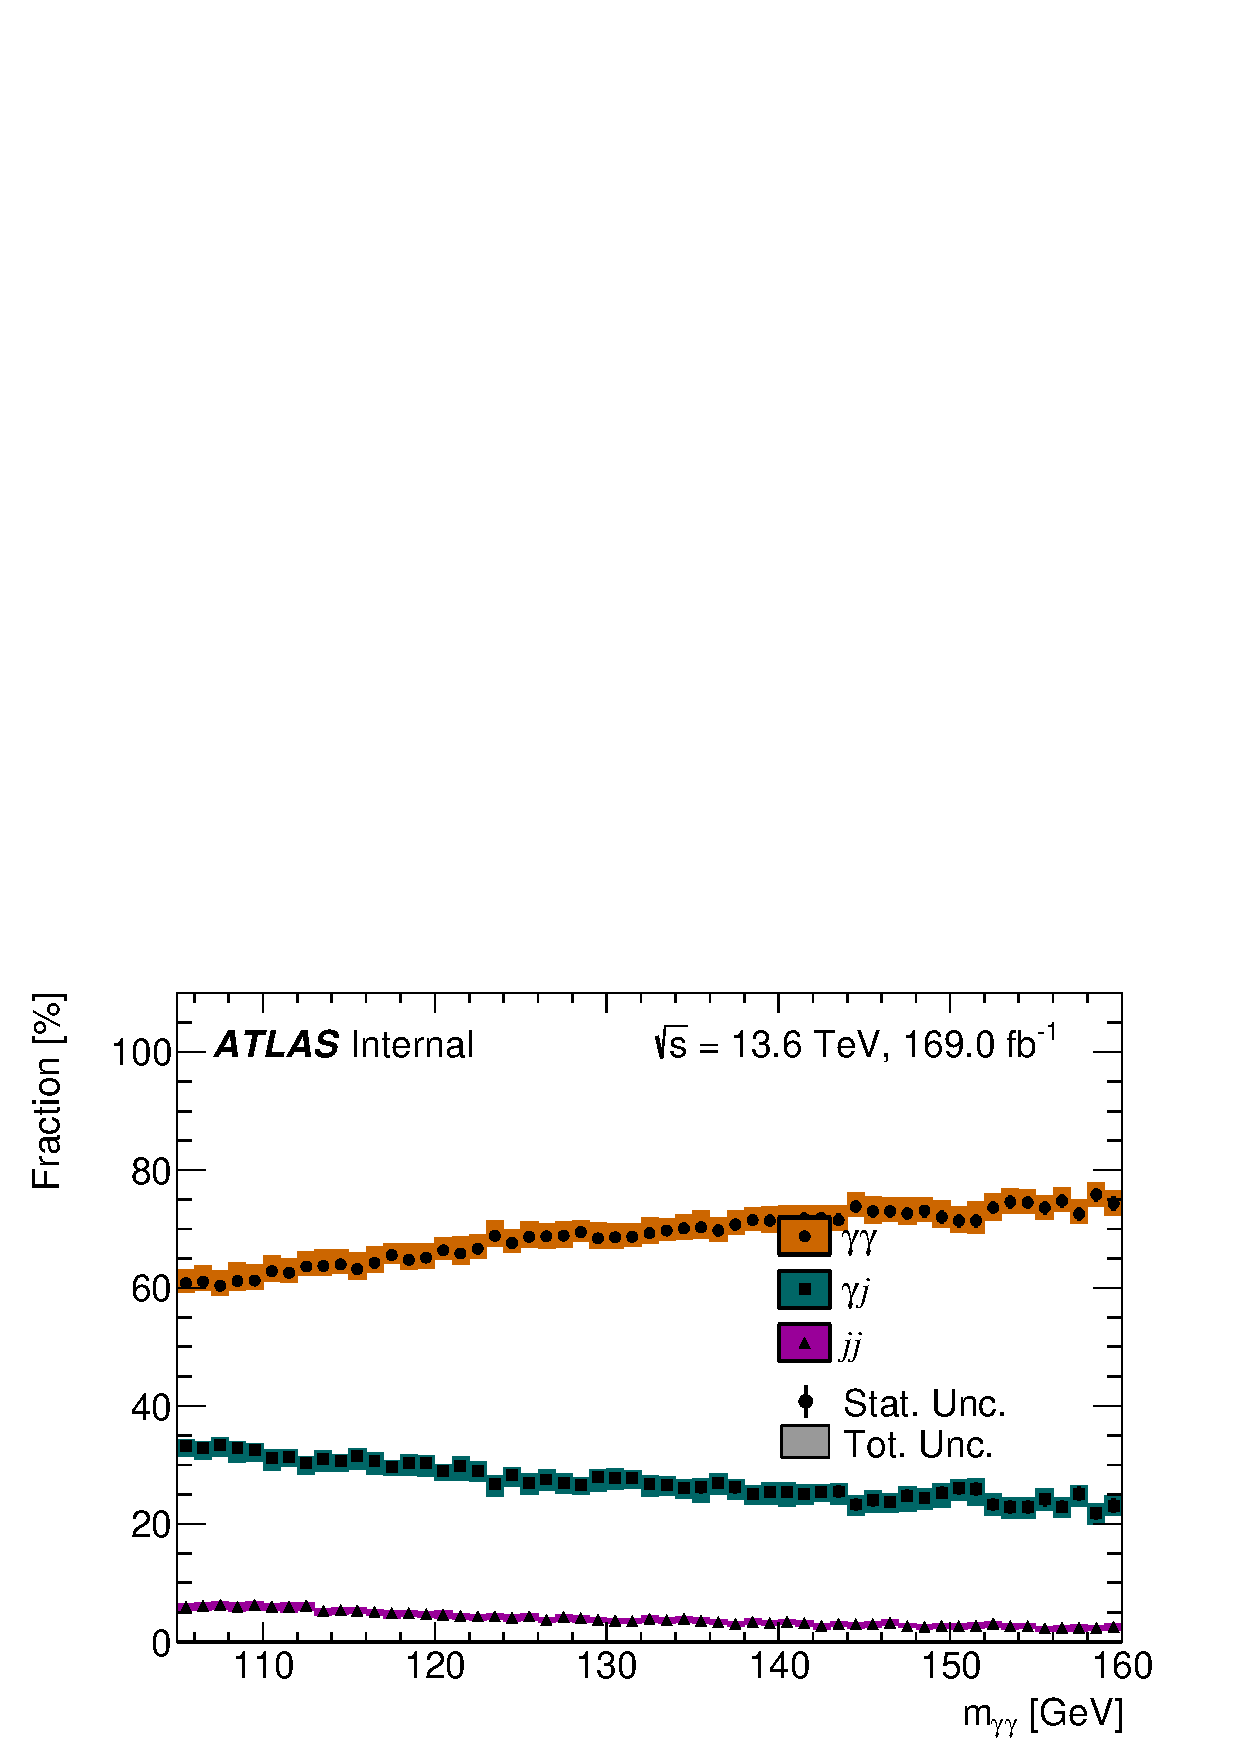
\includegraphics[width=\textwidth]{figures/2x2d_sidebands/plots_sb_diffxsvars_20250930/plot_purity_m_yy.pdf}
        \caption{}
        \label{fig:2x2dpurmyy202224}
    \end{subfigure}
    \begin{subfigure}{0.49\textwidth}
        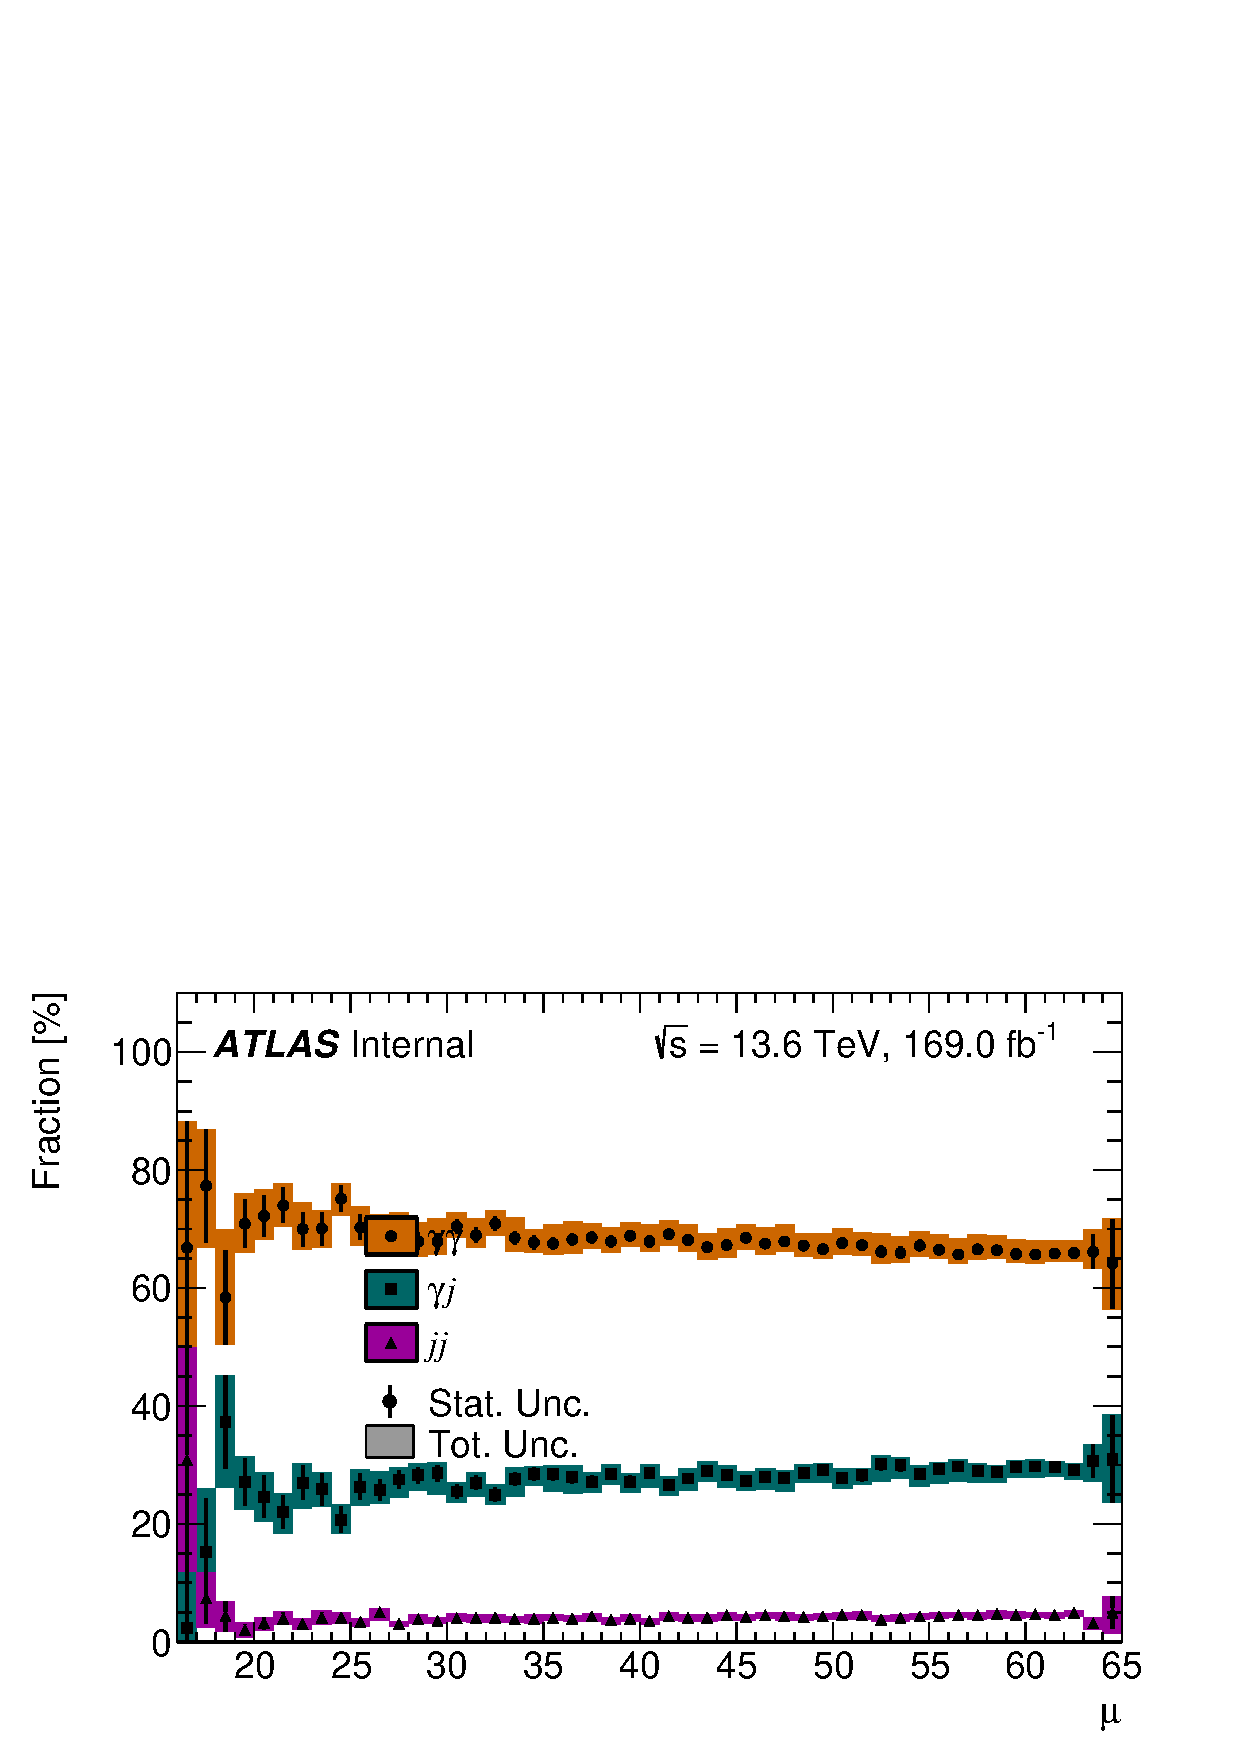
\includegraphics[width=\textwidth]{figures/2x2d_sidebands/plots_sb_diffxsvars_20250930/plot_purity_mu.pdf}
        \caption{}
        \label{fig:2x2dpurmu202224}
    \end{subfigure}
    \begin{subfigure}{0.49\textwidth}
        \centering
        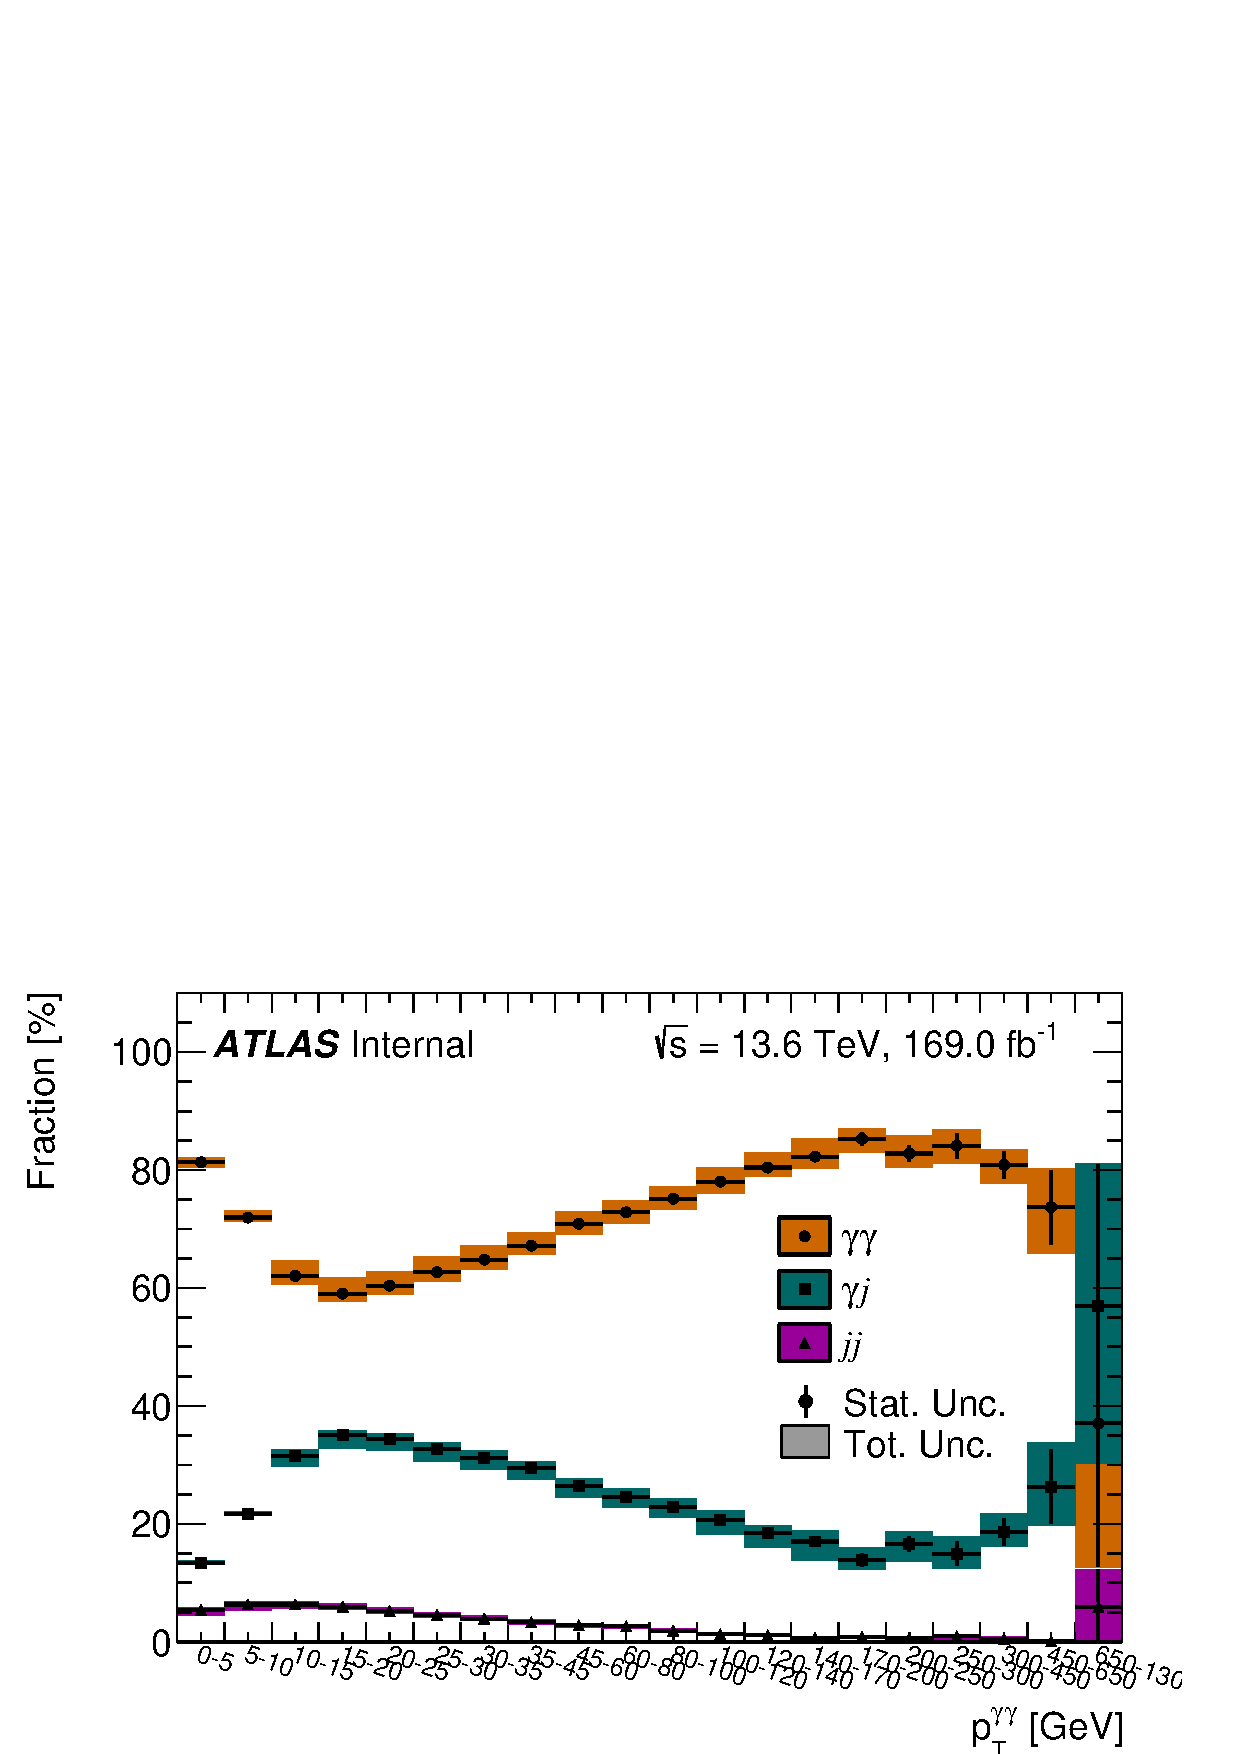
\includegraphics[width=\textwidth]{figures/2x2d_sidebands/plots_sb_diffxsvars_20250930/plot_purity_pT_yy.pdf}
        \caption{}
        \label{fig:2x2dpurptyy202224}
    \end{subfigure}
    \caption{Background purity for 2022--2024 data (\texttt{mc23a--e}) for (a) inclusive events ($105 < m_{\gamma \gamma} < 160$ GeV), (b) $m_{\gamma \gamma}$, (c) $\mu$, and (d) $p_{\mathrm{T}}^{\gamma \gamma}$.}
    \label{fig:2x2dpurity202224:1}
\end{figure}


\begin{figure}[!h]
    \centering
    \begin{subfigure}{0.49\textwidth}
        \centering
        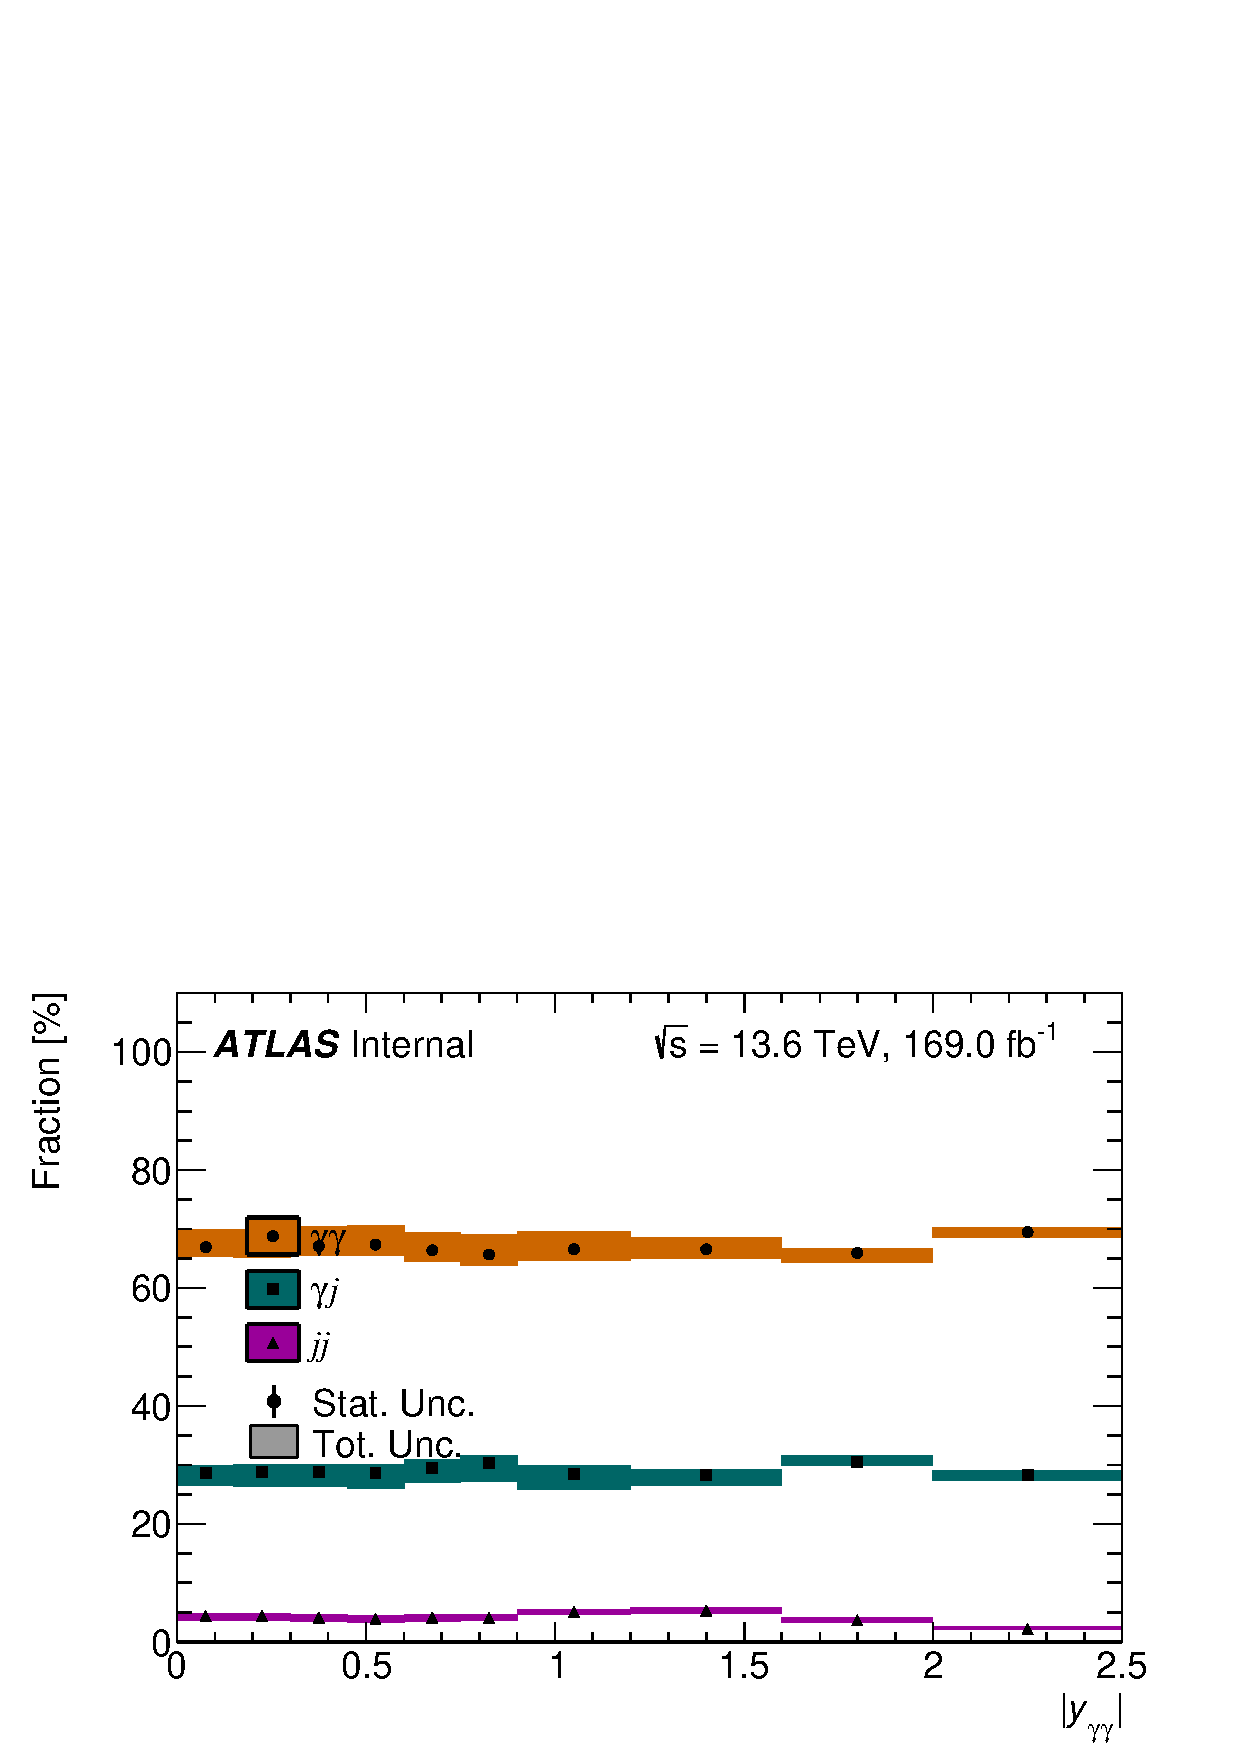
\includegraphics[width=\textwidth]{figures/2x2d_sidebands/plots_sb_diffxsvars_20250930/plot_purity_yAbs_yy.pdf}
        \caption{}
        \label{fig:2x2dpuryabsyy202224}
    \end{subfigure}
    \begin{subfigure}{0.49\textwidth}
        \centering
        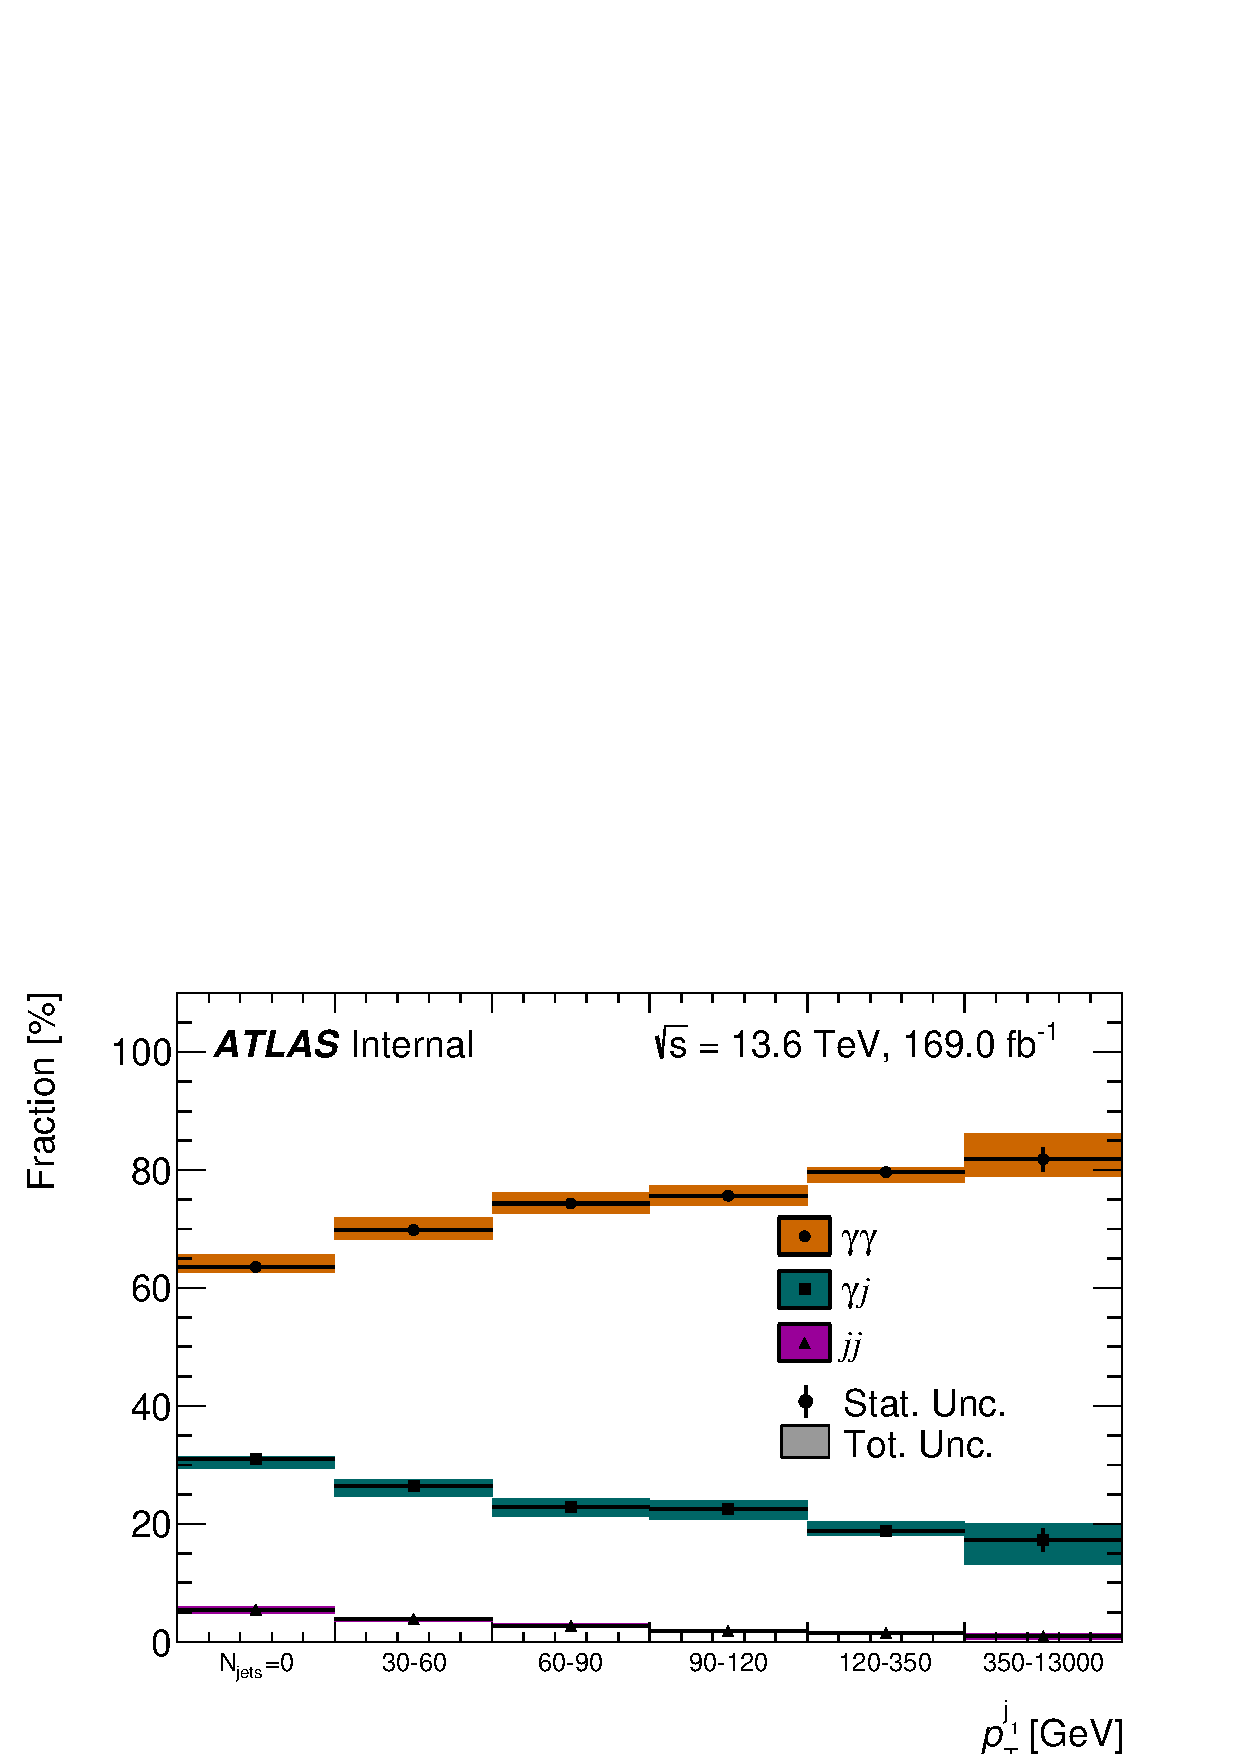
\includegraphics[width=\textwidth]{figures/2x2d_sidebands/plots_sb_diffxsvars_20250930/plot_purity_pT_j1_30.pdf}
        \caption{}
        \label{fig:2x2dpurptj1202224}
    \end{subfigure}
    \begin{subfigure}{0.49\textwidth}
        \centering
        \includegraphics[width=\textwidth]{figures/2x2d_sidebands/plots_sb_diffxsvars_20250930/plot_purity_N_j_30.pdf}
        \caption{}
        \label{fig:2x2dpurnjets202224}
    \end{subfigure}
    \begin{subfigure}{0.49\textwidth}
        \centering
        \includegraphics[width=\textwidth]{figures/2x2d_sidebands/plots_sb_diffxsvars_20250930/plot_purity_m_jj_30.pdf}
        \caption{}
        \label{fig:2x2dpurmjj202224}
    \end{subfigure}
    \caption{Background purity for 2022--2024 data (\texttt{mc23a--e}) as a function of (a) $|y_{\gamma \gamma}|$, (b) $p_{\mathrm{T}}^{j_1}$, (c) $N_{\mathrm{jets}}$, and (d) $m_{jj}$.}
    \label{fig:2x2dpurity202224:2}
\end{figure}


\begin{figure}[!h]
    \centering
    \begin{subfigure}{0.49\textwidth}
        \centering
        \includegraphics[width=\textwidth]{figures/2x2d_sidebands/plots_sb_diffxsvars_20250930/plot_purity_Dphi_j_j_30_signed.pdf}
        \caption{}
        \label{fig:2x2dpurdphijj202224}
    \end{subfigure}
    \begin{subfigure}{0.49\textwidth}
        \centering
        \includegraphics[width=\textwidth]{figures/2x2d_sidebands/plots_sb_diffxsvars_20250930/plot_purity_N_j_btag30.pdf}
        \caption{}
        \label{fig:2x2dpurnbjets202224}
    \end{subfigure}
    \begin{subfigure}{0.49\textwidth}
        \centering
        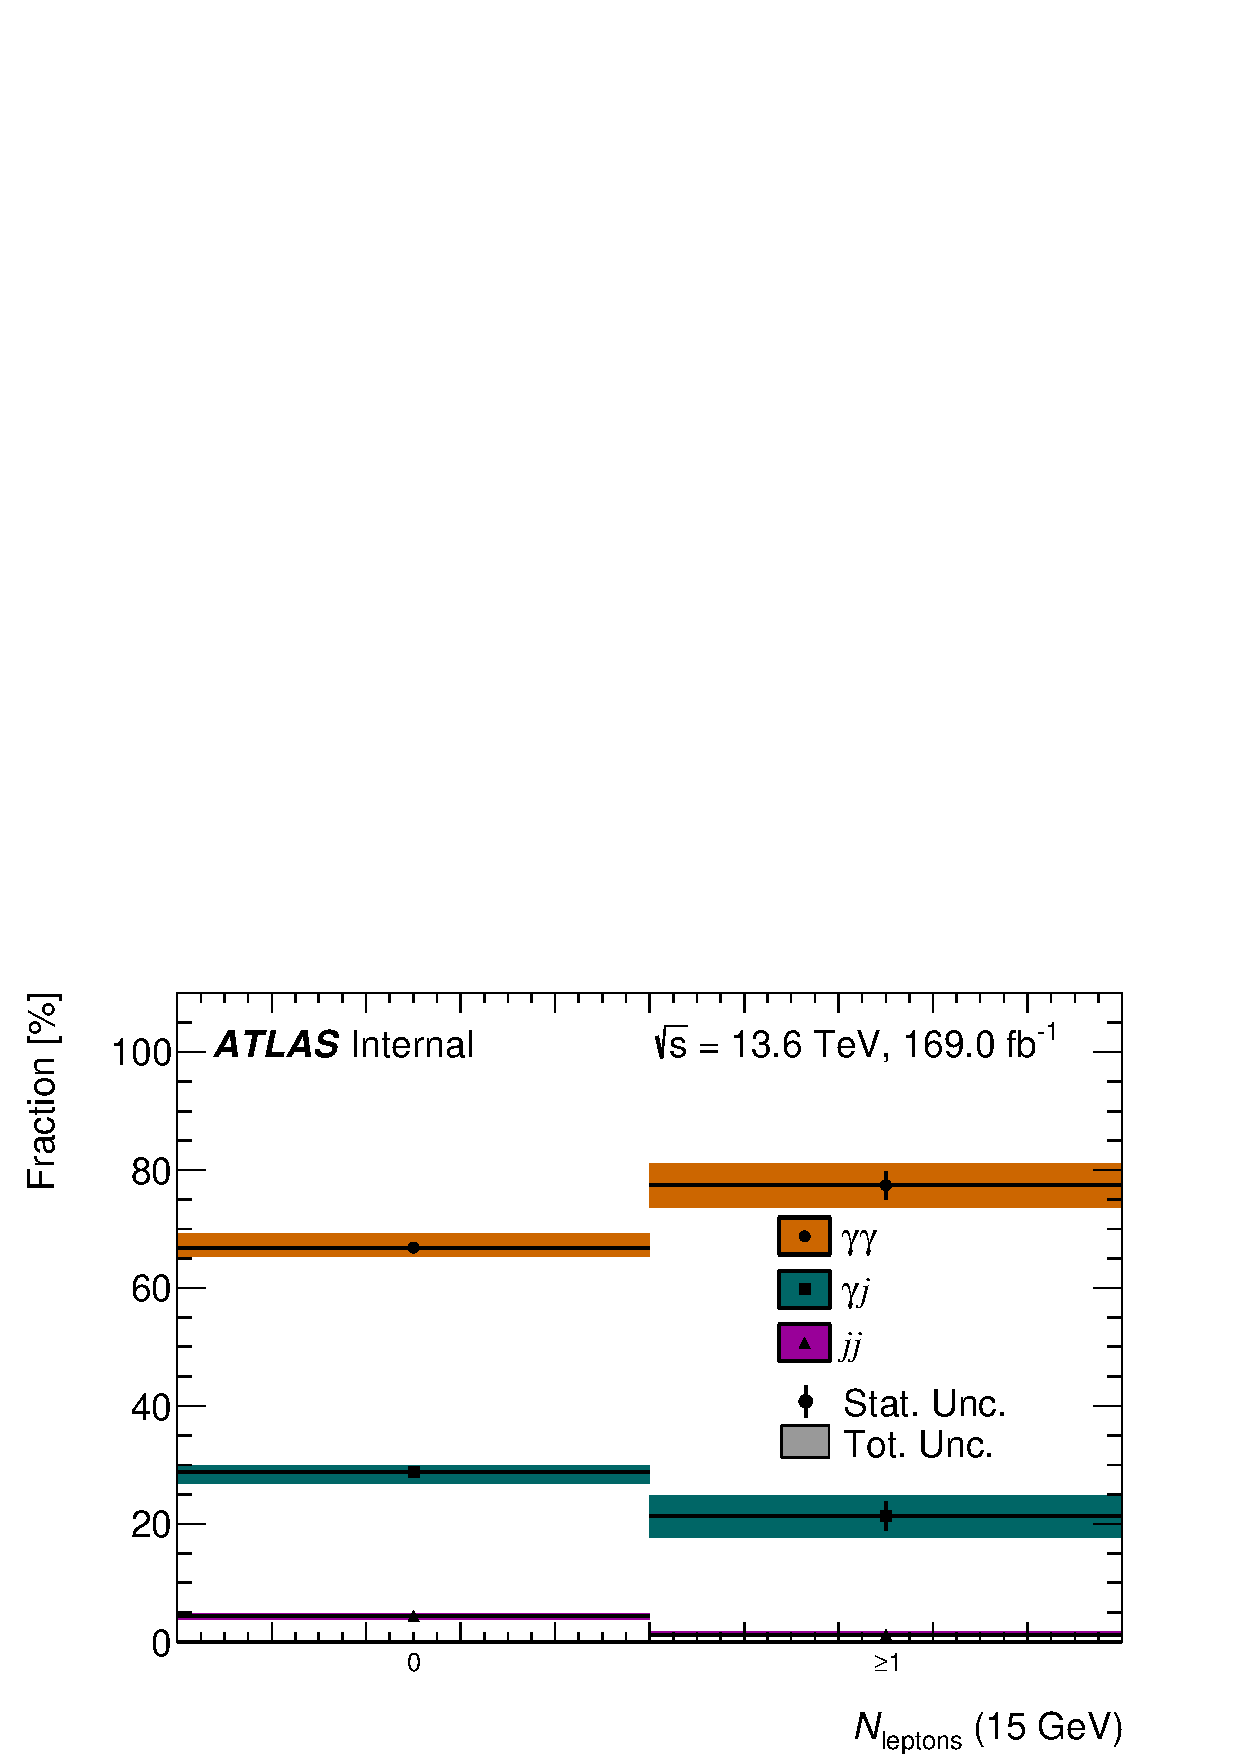
\includegraphics[width=\textwidth]{figures/2x2d_sidebands/plots_sb_diffxsvars_20250930/plot_purity_N_lep_15.pdf}
        \caption{}
        \label{fig:2x2dpurnlept202224}
    \end{subfigure}
    \caption{Background purity for 2022--2024 data (\texttt{mc23a--e}) as a function of (a) $\Delta \phi_{jj}$, (b) $N_{\mathrm{b-jets}}$, and (c) $N_{\mathrm{leptons}}$.}
    \label{fig:2x2dpurity202224:3}
\end{figure}



\section{Uncertainties}
\label{sec:uncertainties}

The main systematic uncertainties affecting the differential cross-section measurements can be divided into two sources, theoretical and experimental.
The theoretical uncertainties include the QCD scale, parton density functions, the value of the strong coupling constant and branching ratios.
Most of these uncertainties can cause migrations between different bins and are therefore computed as uncertainties on the efficiency and the acceptance for each observable.

\textcolor{blue}{This needs to be revisited when we update the results to h033} Experimental uncertainties act both on the signal yield and shape. 
The main uncertainties on the yield originate from the spurious signal, the measured integrated luminosity, trigger efficiency and Higgs mass, pileup-reweighting, the selection of the primary vertex, as well as photon identification and isolation. 
Uncertainties on event migration include jet uncertainties, lepton efficiency and ID, $E_T^{miss}$, flavour tagging and pileup-reweighting. 
Finally, uncertainties on the signal shape are introduced by the photon energy resolution and scale.

\subsection{Experimental Uncertainties}
\label{sec:experimentaluncertainties}

\subsubsection{Signal shape uncertainties}
\label{sssec:signal_shape_syst}

The photon energy scale (PES) and the photon energy resolution (PER) variations act both on the signal shape and on the overall yields. 
Their effect is included in the fit to data as response functions on $\mu_\text{CB}$ and $\sigma_\text{CB}$, respectively. 
The remaining parameters of the Double Sided Crystal Ball function used to model the signal are kept constant. 
These systematic variations are extracted for each analysis category and are treated as fully correlated among categories. 
All categories in this analysis are expected to be more sensitive to the PER than to the PES, since the change in the signal width affects the S/B ratio. 

The uncertainties are computed from MC signal samples with all production processes merged according to the predicted SM fractions, using the following techniques:
\begin{itemize}
	\item for the \textbf{scale}, the ratio-of-means technique is used: the mean \myy is computed for the nominal and $\pm 1 \sigma$ varied distributions. Then, the systematic uncertainty applied to $\mu_\text{CB}$ is calculated as
	\begin{equation}
	\delta \mu_\text{CB}^{\pm 1 \sigma} = \frac{\left\langle m_{\gamma\gamma}^{\pm 1 \sigma}\right\rangle}{\left\langle m_{\gamma\gamma}^\text{nom}\right\rangle}-1.
	\end{equation}
	Scale uncertainties are implemented in the fit to the data with a Gaussian constraint using the $+1\sigma$ variation, because of the high degree of symmetry observed in the uncertainties. All the constraints are multiplied together and applied to $\mu_\text{CB}$ as a response function. The shift in the signal peak is usually below 0.3\%, depending on the category under consideration, with the greatest contribution usually being the L2 Gain systematic. Plots for each category are shown in \textcolor{blue}{Plots to be included using h033};
	\item for the \textbf{resolution}, the ratio of inter-quartile ranges is used: the inter-quartile range is computed as $S = \text{CDF}^{-1}(75\%) - \text{CDF}^{-1}(25\%)$, where CDF is the cumulative distribution function of the \myy nominal and varied distributions. Then, the uncertainty is evaluated as
	\begin{equation}
	\delta \sigma_\text{CB}^{\pm 1 \sigma} = \frac{S^{\pm 1 \sigma}}{S^\text{nom}}-1.
	\end{equation}
	Resolution uncertainties are implemented in the fit with an asymmetric constraint, to take into account differences in the up/down components. All the resolution constraints are multiplied together and applied to $\sigma_\text{CB}$ as a response function. The effect of the PER uncertainty on the signal resolutions is typically between 1 and 8\%. \textcolor{blue}{Plots to be included using h033}.
\end{itemize}
%The list of the systematic uncertainties could be found in the \appendixname~\ref{app:ExpSysShape}\\

%\paragraph{Correlation model} Two models are provided by the calibration group: the first with 2 nuisance parameters (one for the scale and one for the resolution uncertainties), the latter with 80 systematics sources, 71 of which dedicated to scale uncertainties. As in the previous analysis, we will be able to constrain the 1NP model, so we have to go for the full one: in particular, we use a full decorrelated model for the resolution (9 NPs) and a merged one for the scale (40 NPs, since we are not so sensitive to scale variations): the NPs related to the material in front of the calorimeter (MATCALO and MATCRYO), to the presampler (PS) and to S12, which are divided in many $\eta$ bins, are sum together in two contributions each, one bin for the barrel and one for the endcap region.
\subsubsection{Signal yield uncertainties}
\label{sssec:signal_yield_syst}

Yield uncertainties act on the yield of a given reconstructed category, letting events migrate among them or changing the efficiency of the diphoton selection. 
Various experimental systematic sources relating to the photon selections are taken into account: photon uncertainties on \textit{isolation} and \textit{identification} efficiency, uncertainties on the efficiency of the diphoton \textit{trigger} and from \textit{pileup} modelling in simulation. 
From additional objects present in all the categories, the main experimental systematic sources of uncertainty are jet reconstruction uncertainties, especially jet flavour composition, flavour response, modelling, topology and jet energy resolution.
From per-event computed quantities, the dominant sources are the pileup reweighing (PRW) and the luminosity measurement. Both these uncertainties are fully correlated between all bins in all fiducial regions. 
The values for each category \emph{c} are computed as the relative difference between $\pm1\sigma$ varied yields and the nominal one using signal MC samples: 
\begin{equation}
\delta n_{c}^{\pm 1 \sigma} = \frac{n_{c}^{\pm 1 \sigma}}{n_{c}^\text{nom}} - 1
\label{eq:yield_syst}
\end{equation}
Each source of systematic uncertainty is treated as fully correlated within the categories. The nuisance parameters corresponding to these systematic uncertainties are entered into the fit with asymmetric constraints, as the up- and down-variations can  take different values. 
\textcolor{blue}{Plots to be included using h033}.







\subsection{Theory Model Uncertainties}
\label{sec:modellinguncertainties}
Uncertainties due to the theoretical modelling of particle physics processes are evaluated using Monte Carlo predictions. The main sources of theoretical systematic uncertainty are described in this section. Details of the alternative Monte Carlo samples and configurations have been provided in Section \ref{sec:samples}.

\paragraph{QCD scale} The QCD scale uncertainties are obtained using nine-point scale variations of the NLO renormalisation and factorisation scales and applying the NNLO reweighting to those variations, including up and down variations of $\mu_\text{R} = \mu_\text{F}$ around the central value for the NNLO part, yielding a total of 27 scale variations.
%Uncertainties related to the choice of the QCD scale are estimated by varying the renormalisation and factorisation scales independently by factors of 0.5 and 2.  

\paragraph{PS+Hadronisation} Uncertainty due to the modelling of parton showers and hadronisation is estimated using alternative MC predictions using Herwig 7.2.3 \cite{Bellm:2015jjp,Bellm:2020epjc}. These alternative samples use the same matrix element generators as the nominal samples. Herwig 7.2 uses an angular-ordered parton shower and a cluster-based hadronisation model, as opposed to the \pT-ordered dipole shower and Lund-string hadronisation used in Pythia 8.  

\paragraph{PDF} Uncertainties due to the choice of parton distribution functions (PDFs) and \alphas are estimated using the \PDFforLHC[15nlo] set of eigenvectors\cite{Butterworth:2015oua}. The uncertainty is computed as the envelope of all eigenvector variations in the PDF set.

\textcolor{red}{TODO: Add descriptions of more uncertainties as samples become available.} 

\textcolor{red}{TODO: Add summary of impact of theoretical uncertainties on the final results.} 

\section{Unfolding}
\label{sec:unfolding}

\section{Signal Yield Extraction}
\label{sec:signalyieldextraction}
\section{Expected Results (Asimov Dataset)}
\label{sec:asimovresults}

Using the Asimov dataset described in Section \ref{ssec:asimov} expected cross-sections and their uncertainties are
extracted. This provides:
\begin{enumerate}
\item Checks of the signal yield extraction; do the cross-sections match the injected SM predictions?
\item Means to investigate systematic uncertainties. In particular, as the uncertainties experience no pulls and constraints in Asimov dataset fits, 
any unexpected trends should be traced to their source.  
\end{enumerate}
The results are shown for each of Bin-by-bin Corrections in Section \ref{ssec:asimovresults_bin_by_bin} (available now) and for
Matrix-Inversion Unfolding in Section \ref{ssec:asimovresults_mi} (to be filled once available).

\subsection{Expected Results Using Bin-by-bin Corrections}
\label{ssec:asimovresults_bin_by_bin}
 
\begin{figure}[htb!]
  \begin{center}
 \includegraphics[width=0.4\textwidth]{figures/results_wonky_format/bin_by_bin/AsimovSB/Diphoton/constant/plot_Diphoton_constant.png} 
 \includegraphics[width=0.4\textwidth]{figures/results_wonky_format/bin_by_bin/AsimovSB/VBF/constant/plot_VBF_constant.png}
  \end{center}
  \caption{Expected cross-sections from bin-by-bin unfolding, for the inclusive Diphoton (left) and VBF (right) selections. The 
  SM predictions are shown in a full line, and the expected result as filled circles. The error bars are shown 
for each of the total (statistics+systematics) and statistics-only uncertainties.}
  \label{fig:plot_bin_by_bin_AsimovSB_1}
\end{figure}

\begin{figure}[htb!]
  \begin{center}
 \includegraphics[width=0.32\textwidth]{figures/results_wonky_format/bin_by_bin/AsimovSB/MET/constant/plot_MET_constant.png} 
 \includegraphics[width=0.32\textwidth]{figures/results_wonky_format/bin_by_bin/AsimovSB/Lepton/constant/plot_Lepton_constant.png}
  \includegraphics[width=0.32\textwidth]{figures/results_wonky_format/bin_by_bin/AsimovSB/ttH/constant/plot_ttH_constant.png}
  \end{center}
  \caption{Same as Figure~\ref{fig:plot_bin_by_bin_AsimovSB_1} but for MET (left) and Lepton (middle) and ttH (right) selections.}
  \label{fig:plot_bin_by_bin_AsimovSB_2}
\end{figure}
  
Figures \ref{fig:plot_bin_by_bin_AsimovSB_1}--\ref{fig:plot_bin_by_bin_AsimovSB_diff_3} provide checks of 
point 1) \textit{do the cross-sections match the injected SM predictions?} Specifically, the cross-sections should match the SM prediction times 
the relevant correction factor, as described in Section \ref{ssec:asimov}. The cross-sections in all figures are shown without 
the \hgg{} branching ratio. 

Figures \ref{fig:plot_bin_by_bin_AsimovSB_1} and \ref{fig:plot_bin_by_bin_AsimovSB_2} show the results for the inclusive selections, 
matching the injected values of: 29.8 fb for Diphoton, 0.626 fb for VBF, 0.134 fb for MET, 0.271 fb for Lepton and 0.271 fb for the ttH region. 
Consequently, the values in the bottom panels of the figures, which show the ratio of the injected and extracted cross-sections, are equal to 1.
The Lepton and ttH regions happen to have the same cross-sections within the rounding uncertainty, and the sub-process composition has been checked 
to verify this is a numerical coincidence rather than a bug. Spefically, as expected the ttH region contributions are predominantlt from the ttH production, 
whereas the Lepton region also has large contributions from the WH and ZH production. 
% R2 vs R3 with BR 
%ggH & 0.06360321988522163 & 0.06780961838061474
%VBF & 0.001314668111586092 & 0.0014211190061389895
%MET & 0.0002939593517821063 & 0.00030333575875796256
%Lepton & 0.0005671117028774617 & 0.0006154765838685054
%ttH    & /                     & 0.0006151611831697103

The figures also show the expected uncertainty, as a total (statistics+systematics) and statistics-only uncertainties. In all cases, statistics 
uncertainty contribution is sizeable. In the current iteration of the plots done with h032 samples, only a simplified uncertainty scheme could be used, 
and all results currently lack the theory modelling uncertainties. Once these are included, the statistics and systematics uncertainties will become more 
comparable, especially for the Diphoton selection. 


Figures \ref{fig:plot_bin_by_bin_AsimovSB_diff_1}--\ref{fig:plot_bin_by_bin_AsimovSB_diff_3} 
show the results for the differential distributions. The bottom panels likewise confirm that the extracted cross-sections  match the injected ones.  
For the differential distributions, the binning has been designed to reach the expected significance of about 2-$\sigma$ in most bins, as detailed in 
Section \ref{sec:binningoptimisation}. This criterion means that all bins are dominated by the statistical uncertainty. This will remain the case also 
once a complete set of systematics uncertainties is taken into account. 

\begin{figure}[htb!]
  \begin{center}
 \includegraphics[width=0.4\textwidth]{figures/results_wonky_format/bin_by_bin/AsimovSB/Diphoton/pT_yy/plot_Diphoton_pT_yy.png} 
\includegraphics[width=0.4\textwidth]{figures/results_wonky_format/bin_by_bin/AsimovSB/Diphoton/yAbs_yy/plot_Diphoton_yAbs_yy.png}
  \end{center}
  \caption{Expected cross-sections from bin-by-bin unfolding for the inclusive Diphoton selection and the \ptgg{} and \ygg{} distributions.
   The 
  SM predictions are shown in a full line, and the expected result as filled circles. The error bars are shown 
for each of the total (statistics+systematics) and statistics-only uncertainties.
  }
  \label{fig:plot_bin_by_bin_AsimovSB_diff_1}
\end{figure}

\begin{figure}[htb!]
  \begin{center}
 \includegraphics[width=0.32\textwidth]{figures/results_wonky_format/bin_by_bin/AsimovSB/Diphoton/m_jj_30/plot_Diphoton_m_jj_30.png}
\includegraphics[width=0.32\textwidth]{figures/results_wonky_format/bin_by_bin/AsimovSB/Diphoton/Dphi_j_j_30_signed/plot_Diphoton_Dphi_j_j_30_signed.png}
\includegraphics[width=0.32\textwidth]{figures/results_wonky_format/bin_by_bin/AsimovSB/Diphoton/pT_j1_30/plot_Diphoton_pT_j1_30.png}
  \end{center}
  \caption{Same as Figure~\ref{fig:plot_bin_by_bin_AsimovSB_diff_1} but for the \dphijj{}, \mjj{} and \ptj{} distributions.}
  \label{fig:plot_bin_by_bin_AsimovSB_diff_2}
\end{figure}

\begin{figure}[htb!]
  \begin{center}
 \includegraphics[width=0.32\textwidth]{figures/results_wonky_format/bin_by_bin/AsimovSB/Diphoton/N_j_30/plot_Diphoton_N_j_30.png}
\includegraphics[width=0.32\textwidth]{figures/results_wonky_format/bin_by_bin/AsimovSB/Diphoton/N_lep_15/plot_Diphoton_N_lep_15.png}
\includegraphics[width=0.32\textwidth]{figures/results_wonky_format/bin_by_bin/AsimovSB/Diphoton/N_j_btag30/plot_Diphoton_N_j_btag30.png}
  \end{center}
  \caption{Same as Figure~\ref{fig:plot_bin_by_bin_AsimovSB_diff_1} but for the  \Njets{}, \Nlept{} and \Nbjets{}
   distributions.}
  \label{fig:plot_bin_by_bin_AsimovSB_diff_3}
\end{figure}


The composition of the total uncertainty for each of the cross-sections can be studies by peforming the signal extraction fits with 
the family of nuisance parameters fixed of allowed to float. For the inclusive fiducial region selections, the results are shown 
for the Diphoton and VBF selections in Figure~\ref{fig:fraction_sys_errorgroup_bin_by_bin_AsimovSB_1} 
and  MET, Lepton and ttH  selections in Figre~\ref{fig:fraction_sys_errorgroup_bin_by_bin_AsimovSB_2}. 
The spurious signal is not visible in the plots, because the injected contributions (taken from Run2 for now) 
are of the order of magnitude $|max(S)/Sref|\sim 0.05$\% for the inclusive selections. With the current uncertainty scheme, 
the luminosity uncertainty taken as 2\% is the single largest contribution to the systematics uncertainty in all but the ttH region. 

\begin{figure}[htb!]
  \begin{center}
 \includegraphics[width=0.4\textwidth]{figures/results_wonky_format/bin_by_bin/AsimovSB/Diphoton/constant/fraction_sys_errorgroup_bin_by_bin_Diphoton_constant.png} 
 \includegraphics[width=0.4\textwidth]{figures/results_wonky_format/bin_by_bin/AsimovSB/VBF/constant/fraction_sys_errorgroup_bin_by_bin_VBF_constant.png}
  \end{center}
  \caption{Fractional uncertainty composition for the inclusive Diphoton (left) and VBF (right) selections. The left axis shows the fractional uncertainty 
with respect to the total systematics uncertainty. The right axis shows the total expected relative uncertainty, also including the statistical uncertainty. 
The display does not really work well and will be updated - the take-away from this right axis is that the total uncertainty is $\sim$ 8\% and 22\% for the 
Diphoton and VBF selections respectively.}
  \label{fig:fraction_sys_errorgroup_bin_by_bin_AsimovSB_1}
\end{figure}

\begin{figure}[htb!]
  \begin{center}
 \includegraphics[width=0.32\textwidth]{figures/results_wonky_format/bin_by_bin/AsimovSB/MET/constant/fraction_sys_errorgroup_bin_by_bin_MET_constant.png} 
 \includegraphics[width=0.32\textwidth]{figures/results_wonky_format/bin_by_bin/AsimovSB/Lepton/constant/fraction_sys_errorgroup_bin_by_bin_Lepton_constant.png}
  \includegraphics[width=0.32\textwidth]{figures/results_wonky_format/bin_by_bin/AsimovSB/ttH/constant/fraction_sys_errorgroup_bin_by_bin_ttH_constant.png}
  \end{center}
  \caption{Same as Figure~\ref{fig:fraction_sys_errorgroup_bin_by_bin_AsimovSB_1} but for MET (left), Lepton (middle) and ttH (right) selections.}
  \label{fig:fraction_sys_errorgroup_bin_by_bin_AsimovSB_2}
\end{figure}

Figures~\ref{fig:fraction_sys_errorgroup_bin_by_bin_bin_by_bin_AsimovSB_diff_1}, \ref{fig:fraction_sys_errorgroup_bin_by_bin_bin_by_bin_AsimovSB_diff_2} and 
\ref{fig:fraction_sys_errorgroup_bin_by_bin_bin_by_bin_AsimovSB_diff_3} show the uncertainty composition for the differential observables. For these, the spurions 
signal is typically the largest single contribution to the systematic uncertainty. 
TODO LM: check what is going on with mjj in Fig \ref{fig:fraction_sys_errorgroup_bin_by_bin_bin_by_bin_AsimovSB_diff_2} - only has 2 bins. 

\begin{figure}[htb!]
  \begin{center}
 \includegraphics[width=0.4\textwidth]{figures/results_wonky_format/bin_by_bin/AsimovSB/Diphoton/pT_yy/fraction_sys_errorgroup_bin_by_bin_Diphoton_pT_yy.png} 
\includegraphics[width=0.4\textwidth]{figures/results_wonky_format/bin_by_bin/AsimovSB/Diphoton/yAbs_yy/fraction_sys_errorgroup_bin_by_bin_Diphoton_yAbs_yy.png}
  \end{center}
  \caption{inclusive Diphoton selection and the \ptgg{} and \ygg{} distributions.}
  \label{fig:fraction_sys_errorgroup_bin_by_bin_bin_by_bin_AsimovSB_diff_1}
\end{figure}

\begin{figure}[htb!]
  \begin{center}
 \includegraphics[width=0.32\textwidth]{figures/results_wonky_format/bin_by_bin/AsimovSB/Diphoton/m_jj_30/fraction_sys_errorgroup_bin_by_bin_Diphoton_m_jj_30.png}
\includegraphics[width=0.32\textwidth]{figures/results_wonky_format/bin_by_bin/AsimovSB/Diphoton/Dphi_j_j_30_signed/fraction_sys_errorgroup_bin_by_bin_Diphoton_Dphi_j_j_30_signed.png}
\includegraphics[width=0.32\textwidth]{figures/results_wonky_format/bin_by_bin/AsimovSB/Diphoton/pT_j1_30/fraction_sys_errorgroup_bin_by_bin_Diphoton_pT_j1_30.png}
  \end{center}
  \caption{Same as Figure~\ref{fig:fraction_sys_errorgroup_bin_by_bin_bin_by_bin_AsimovSB_diff_1} but for the \dphijj{}, \mjj{} and \ptj{} distributions.}
  \label{fig:fraction_sys_errorgroup_bin_by_bin_bin_by_bin_AsimovSB_diff_2}
\end{figure}

\begin{figure}[htb!]
  \begin{center}
 \includegraphics[width=0.32\textwidth]{figures/results_wonky_format/bin_by_bin/AsimovSB/Diphoton/N_j_30/fraction_sys_errorgroup_bin_by_bin_Diphoton_N_j_30.png}
\includegraphics[width=0.32\textwidth]{figures/results_wonky_format/bin_by_bin/AsimovSB/Diphoton/N_lep_15/fraction_sys_errorgroup_bin_by_bin_Diphoton_N_lep_15.png}
\includegraphics[width=0.32\textwidth]{figures/results_wonky_format/bin_by_bin/AsimovSB/Diphoton/N_j_btag30/fraction_sys_errorgroup_bin_by_bin_Diphoton_N_j_btag30.png}
  \end{center}
  \caption{Same as Figure~\ref{fig:fraction_sys_errorgroup_bin_by_bin_bin_by_bin_AsimovSB_diff_1} but for the  \Njets{}, \Nlept{} and \Nbjets{}
   distributions.}
  \label{fig:fraction_sys_errorgroup_bin_by_bin_bin_by_bin_AsimovSB_diff_3}
\end{figure}

Finally, for the differential distributions, the correlations between the bins of the extracted cross-sections can be checked. 
The bin-by-bin corrections used in this section neglects the migration between the bins, 
and therefore the results are only expected to be close to more sophisticated unfolding methods, 
such as the matrix inversion unfolding described in Section \ref{ssec:asimovresults_mi}, 
for observables with roughly diagonal correlation 
matrices, such as \ptgg{} and \ygg{}. For observables with non-diagonal correlation matrices, such as jet-related observables, 
the extracted correlations are instead not representative of what's expected from the matrix inversion unfolding.
Due to these caveats, the correlations are only shown for two representative distributions in Figures \ref{fig:correlation_bin_by_bin_AsimovSB_diff_1}: 
\ygg{} with rouhgly diagonal correlation matrix and Njets with non-diagonal correlation matrix. 

\begin{figure}[htb!]
  \begin{center}
 \includegraphics[width=0.45\textwidth]{figures/results_wonky_format/bin_by_bin/AsimovSB/Diphoton/yAbs_yy/correlation_Diphoton_yAbs_yy_full.png}
 \includegraphics[width=0.45\textwidth]{figures/results_wonky_format/bin_by_bin/AsimovSB/Diphoton/N_j_30/correlation_Diphoton_N_j_30_full.png}
  \end{center}
  \caption{Correlations between the bins of the extracted cross-sections for the \ptgg{} (left) and Njets (right) distributions.}
  \label{fig:correlation_bin_by_bin_AsimovSB_diff_1}
\end{figure}

\subsection{Expected Results Using Matrix-Inversion Unfolding}
\label{ssec:asimovresults_mi}
\section{Results (Run 3 Data) [PENDING UNBLINDING]}
\label{sec:dataresults} %After unblinding

\section{Conclusion}
\label{sec:conclusion}

Measurements of Higgs boson fiducial cross-sections in the diphoton decay channel are performed using \pp\ collision data recorded by the ATLAS experiment at the LHC, assuming the Higgs boson mass to be \SI{125.09}{\GeV}.
The data were taken at a centre-of-mass energy of \(\sqrt{s}=\SI{13.6}{\TeV}\) and correspond to the partial Run 3 data set collected between 2022 and 2024 with an integrated luminosity of \SI{165.2}{\femto\barn^{-1}}.

The measurements are performed in a diphoton fiducial region requiring two isolated photons with transverse momentum greater than 35\% and 25\% of the diphoton invariant mass, and with \(|\eta|<2.37\), excluding the region of \(1.37 < |\eta|<1.52\).
The inclusive fiducial cross-section times branching ratio is measured to be \textcolor{red}{to be filled}
%\begin{align*}
%\sigma_\textrm{fid} = 67\pm5~\text{(stat.)}\pm4~\text{(sys.)}~~\si{\femto\barn},
%\end{align*}
%which is in agreement with the Standard Model prediction of \SI[multi-part-units=single]{64\pm 4}{\femto\barn}. The measurement has a total relative uncertainty of 10\% with nearly equal contributions from the statistical and the systematic uncertainties.
%The inclusive fiducial cross-section is also extrapolated to the full phase space, leading to a total Higgs production cross-section of \(58 \pm 4~\text{(stat.)} \pm 4~\text{(sys.)}~\si{\pico\barn}\), in agreement with the SM prediction of \SI[multi-part-units=single]{55.6 \pm 2.7}{\pico\barn}.

In addition, cross-section measurements are reported in various fiducial regions probing Higgs boson production from vector-boson fusion or associated with large missing transverse momentum, leptons or top quarks. The measured cross-sections times branching ratio for the these fiducial regions are: \textcolor{red}{to be filled}
%\begin{align*}
%\sigma_\text{VBF-enhanced}       & = 1.8~~\pm0.5~~~\text{(stat.)} \pm0.3~~~\text{(sys.)}~~\si{\femto\barn}, \\
%\sigma_{N_{\text{lepton} \geq 1}} & = 0.81 \pm0.23~\text{(stat.)} \pm0.06~\text{(sys.)}~~\si{\femto\barn}, \\
%\sigma_{\text{High \met}}             & = 0.28  \pm0.27~\text{(stat.)} \pm0.07~\text{(sys.)}~~\si{\femto\barn}, \\
%\sigma_\text{\ttH-enhanced}        &= 0.53 \pm0.27~\text{(stat.)} \pm0.06~\text{(sys.)}~~\si{\femto\barn}, \\
%\end{align*}
%which show no significant deviation from the Standard Model predictions. The fiducial cross-sections for different inclusive and exclusive jet multiplicities are also measured and compared with different state-of-the-art Standard Model predictions.

Several differential cross-sections are reported for events belonging to the inclusive diphoton fiducial region, as a function of kinematic variables of the diphoton system or of jets produced in association with the Higgs boson. 
These cross-sections are sensitive to the different Higgs boson production kinematics, jet kinematics, spin, and CP quantum numbers of the Higgs boson. Among the measured cross-sections is a new measurement of the cross-section in the high Higgs boson transverse momentum region compared to the Run 2 result \textcolor{red}{TBC}, providing the strongest limits to date for the Higgs boson production cross-section above \SI{600}{\GeV}\textcolor{red}{TBC}. 
%The reported cross-sections include new measurements in regions of the phase space probing jet-veto resummation effects. In addition, four differential cross-sections and one double-differential cross-section were measured for events belonging to the VBF-enhanced region, probing VBF kinematics and CP properties. All the measured differential cross-sections are compared with various Standard Model predictions, and do not exhibit significant deviations from them.




% All figures and tables should appear before the summary and conclusion.
% The package placeins provides the macro \FloatBarrier to achieve this.
% \FloatBarrier

%-------------------------------------------------------------------------------
% If you use biblatex and either biber or bibtex to process the bibliography
% just say \printbibliography here.
\printbibliography
% If you want to use the traditional BibTeX you need to use the syntax below.
% \bibliographystyle{obsolete/bst/atlasBibStyleWithTitle}
% \bibliography{ANA-HIGP-2024-02-INT1,bib/ATLAS,bib/CMS,bib/ConfNotes,bib/PubNotes}
%-------------------------------------------------------------------------------

%-------------------------------------------------------------------------------
% Print the list of contributors to the analysis.
% The argument gives the fraction of the text width used for the names.
%-------------------------------------------------------------------------------
\clearpage
The supporting notes for the analysis should also contain a list of contributors.
This information should usually be included in \texttt{mydocument-metadata.tex}.
The list should be printed either here or before the Table of Contents.
%\PrintAtlasContribute{0.30}

%-------------------------------------------------------------------------------
\clearpage
\appendix
\part*{Appendices}
\addcontentsline{toc}{part}{Appendices}

\section{List of used DAODs}
\label{app:DAODs}

The DAODs used in the analysis are listed below.

\subsection{Data sample}
\tiny
\begin{itemize}
    \item
\detokenize{data22_13p6TeV.periodAllYear.physics_Main.PhysCont.DAOD_HIGG1D1.grp22_v01_p6456}
    \item
\detokenize{data23_13p6TeV.periodAllYear.physics_Main.PhysCont.DAOD_HIGG1D1.grp23_v01_p6456}
    \item 
\detokenize{data24_13p6TeV.periodAllYear.physics_Main.PhysCont.DAOD_HIGG1D1.grp24_v01_p6456}
\end{itemize}


\subsection{Nominal signal sample}
\begin{itemize}
  % ggF
  \item \detokenize{mc23_13p6TeV.602421.PhPy8EG_PDF4LHC21_ggH_NNLOPS_gammagamma.deriv.DAOD_HIGG1D1.e8559_s4162_r14622_p6599}
  \item \detokenize{mc23_13p6TeV.602421.PhPy8EG_PDF4LHC21_ggH_NNLOPS_gammagamma.deriv.DAOD_HIGG1D1.e8559_s4159_r15224_p6599}
  \item \detokenize{mc23_13p6TeV.602421.PhPy8EG_PDF4LHC21_ggH_NNLOPS_gammagamma.deriv.DAOD_HIGG1D1.e8559_s4369_r16083_p6599}

  % VBF
  \item \detokenize{mc23_13p6TeV.601482.PhPy8EG_PDF4LHC21_VBFH125_gammagamma.deriv.DAOD_HIGG1D1.e8559_s4162_r14622_p6599}
  \item \detokenize{mc23_13p6TeV.601482.PhPy8EG_PDF4LHC21_VBFH125_gammagamma.deriv.DAOD_HIGG1D1.e8559_s4159_r15224_p6599}
  \item \detokenize{mc23_13p6TeV.601482.PhPy8EG_PDF4LHC21_VBFH125_gammagamma.deriv.DAOD_HIGG1D1.e8559_s4369_r16083_p6599}

  % WpH
  \item \detokenize{mc23_13p6TeV.601484.PhPy8EG_PDF4LHC21_WpH125J_Wincl_MINLO_gammagamma.deriv.DAOD_HIGG1D1.e8559_s4162_r14622_p6599}
  \item \detokenize{mc23_13p6TeV.601484.PhPy8EG_PDF4LHC21_WpH125J_Wincl_MINLO_gammagamma.deriv.DAOD_HIGG1D1.e8559_s4159_r15224_p6599}
  \item \detokenize{mc23_13p6TeV.601484.PhPy8EG_PDF4LHC21_WpH125J_Wincl_MINLO_gammagamma.deriv.DAOD_HIGG1D1.e8559_s4369_r16083_p6599}

  % WmH
  \item \detokenize{mc23_13p6TeV.601483.PhPy8EG_PDF4LHC21_WmH125J_Wincl_MINLO_gammagamma.deriv.DAOD_HIGG1D1.e8559_s4162_r14622_p6599}
  \item \detokenize{mc23_13p6TeV.601483.PhPy8EG_PDF4LHC21_WmH125J_Wincl_MINLO_gammagamma.deriv.DAOD_HIGG1D1.e8559_s4159_r15224_p6599}
  \item \detokenize{mc23_13p6TeV.601483.PhPy8EG_PDF4LHC21_WmH125J_Wincl_MINLO_gammagamma.deriv.DAOD_HIGG1D1.e8559_s4369_r16083_p6599}

  % ZH
  \item \detokenize{mc23_13p6TeV.601523.PhPy8EG_PDF4LHC21_ZH125J_Zincl_MINLO_gammagamma.deriv.DAOD_HIGG1D1.e8559_s4162_r14622_p6599}
  \item \detokenize{mc23_13p6TeV.601523.PhPy8EG_PDF4LHC21_ZH125J_Zincl_MINLO_gammagamma.deriv.DAOD_HIGG1D1.e8559_s4159_r15224_p6599}
  \item \detokenize{mc23_13p6TeV.601523.PhPy8EG_PDF4LHC21_ZH125J_Zincl_MINLO_gammagamma.deriv.DAOD_HIGG1D1.e8559_s4369_r16083_p6599}

  % ggZH
  \item \detokenize{mc23_13p6TeV.601522.PhPy8EG_PDF4LHC21_ggZH125_Zincl_gammagamma.deriv.DAOD_HIGG1D1.e8559_s4162_r14622_p6599}
  \item \detokenize{mc23_13p6TeV.601522.PhPy8EG_PDF4LHC21_ggZH125_Zincl_gammagamma.deriv.DAOD_HIGG1D1.e8559_s4159_r15224_p6599}
  \item \detokenize{mc23_13p6TeV.601522.PhPy8EG_PDF4LHC21_ggZH125_Zincl_gammagamma.deriv.DAOD_HIGG1D1.e8559_s4369_r16083_p6599}

  % ttH
  \item \detokenize{mc23_13p6TeV.602422.PhPy8EG_PDF4LHC21_ttH125_tincl_gammagamma_1file.deriv.DAOD_HIGG1D1.e8559_s4162_r14622_p6599}
  \item \detokenize{mc23_13p6TeV.602422.PhPy8EG_PDF4LHC21_ttH125_tincl_gammagamma_1file.deriv.DAOD_HIGG1D1.e8559_s4159_r15224_p6599}
  \item \detokenize{mc23_13p6TeV.602422.PhPy8EG_PDF4LHC21_ttH125_tincl_gammagamma_1file.deriv.DAOD_HIGG1D1.e8559_s4369_r16083_p6599}

  % bbH
  \item \detokenize{mc23_13p6TeV.601710.PhPy8EG_PDF4LHC21_4FS_A14NNPDF_bbH_gammagamma.deriv.DAOD_HIGG1D1.e8559_s4162_r14622_p6599}
  \item \detokenize{mc23_13p6TeV.601710.PhPy8EG_PDF4LHC21_4FS_A14NNPDF_bbH_gammagamma.deriv.DAOD_HIGG1D1.e8559_s4159_r15224_p6599}
  \item \detokenize{mc23_13p6TeV.601710.PhPy8EG_PDF4LHC21_4FS_A14NNPDF_bbH_gammagamma.deriv.DAOD_HIGG1D1.e8559_s4369_r16083_p6599}
\end{itemize}


\subsection{Alternative signal sample}
\begin{itemize}
  % ggF
  \item \detokenize{mc23_13p6TeV.604315.PhH7EG_PDF4LHC21_ggH125_NNLOPS_Hgammagamma.deriv.DAOD_HIGG1D1.e8588_s4162_r15540_p6599}
  \item \detokenize{mc23_13p6TeV.604315.PhH7EG_PDF4LHC21_ggH125_NNLOPS_Hgammagamma.deriv.DAOD_HIGG1D1.e8588_s4159_r15530_p6599}
  \item \detokenize{mc23_13p6TeV.604315.PhH7EG_PDF4LHC21_ggH125_NNLOPS_Hgammagamma.deriv.DAOD_HIGG1D1.e8588_s4369_r16083_p6599}

  % VBF
  \item \detokenize{mc23_13p6TeV.604318.PhH7EG_PDF4LHC21_VBFH125_Hgammagamma.deriv.DAOD_HIGG1D1.e8588_s4162_r15540_p6599}
  \item \detokenize{mc23_13p6TeV.604318.PhH7EG_PDF4LHC21_VBFH125_Hgammagamma.deriv.DAOD_HIGG1D1.e8588_s4159_r15530_p6599}
  \item \detokenize{mc23_13p6TeV.604318.PhH7EG_PDF4LHC21_VBFH125_Hgammagamma.deriv.DAOD_HIGG1D1.e8588_s4369_r16083_p6599}

  % WpH
  \item \detokenize{mc23_13p6TeV.604312.PhH7EG_PDF4LHC21_WpH125J_Wincl_MINLO_Hgammagamma.deriv.DAOD_HIGG1D1.e8588_s4162_r15540_p6599}
  \item \detokenize{mc23_13p6TeV.604312.PhH7EG_PDF4LHC21_WpH125J_Wincl_MINLO_Hgammagamma.deriv.DAOD_HIGG1D1.e8588_s4159_r15530_p6599}
  \item \detokenize{mc23_13p6TeV.604312.PhH7EG_PDF4LHC21_WpH125J_Wincl_MINLO_Hgammagamma.deriv.DAOD_HIGG1D1.e8588_s4369_r16083_p6599}

  % WmH
  \item \detokenize{mc23_13p6TeV.604311.PhH7EG_PDF4LHC21_WmH125J_Wincl_MINLO_Hgammagamma.deriv.DAOD_HIGG1D1.e8588_s4162_r15540_p6599}
  \item \detokenize{mc23_13p6TeV.604311.PhH7EG_PDF4LHC21_WmH125J_Wincl_MINLO_Hgammagamma.deriv.DAOD_HIGG1D1.e8588_s4159_r15530_p6599}
  \item \detokenize{mc23_13p6TeV.604311.PhH7EG_PDF4LHC21_WmH125J_Wincl_MINLO_Hgammagamma.deriv.DAOD_HIGG1D1.e8588_s4369_r16083_p6599}

  % ZH
  \item \detokenize{mc23_13p6TeV.604313.PhH7EG_PDF4LHC21_ZH125_Zincl_Hgammagamma.deriv.DAOD_HIGG1D1.e8588_s4162_r15540_p6599}
  \item \detokenize{mc23_13p6TeV.604313.PhH7EG_PDF4LHC21_ZH125_Zincl_Hgammagamma.deriv.DAOD_HIGG1D1.e8588_s4159_r15530_p6599}
  \item \detokenize{mc23_13p6TeV.604313.PhH7EG_PDF4LHC21_ZH125_Zincl_Hgammagamma.deriv.DAOD_HIGG1D1.e8588_s4369_r16083_p6599}

  % ggZH
  \item \detokenize{mc23_13p6TeV.604316.PhH7EG_PDF4LHC21_ggZH125_Zincl_Hgammagamma.deriv.DAOD_HIGG1D1.e8588_s4162_r15540_p6599}
  \item \detokenize{mc23_13p6TeV.604316.PhH7EG_PDF4LHC21_ggZH125_Zincl_Hgammagamma.deriv.DAOD_HIGG1D1.e8588_s4159_r15530_p6599}
  \item \detokenize{mc23_13p6TeV.604316.PhH7EG_PDF4LHC21_ggZH125_Zincl_Hgammagamma.deriv.DAOD_HIGG1D1.e8588_s4369_r16083_p6599}

  % ttH
  \item \detokenize{mc23_13p6TeV.604317.PhH7EG_PDF4LHC21_ttH125_tincl_Hgammagamma.deriv.DAOD_HIGG1D1.e8588_s4162_r15540_p6599}
  \item \detokenize{mc23_13p6TeV.604317.PhH7EG_PDF4LHC21_ttH125_tincl_Hgammagamma.deriv.DAOD_HIGG1D1.e8588_s4159_r15530_p6599}
  \item \detokenize{mc23_13p6TeV.604317.PhH7EG_PDF4LHC21_ttH125_tincl_Hgammagamma.deriv.DAOD_HIGG1D1.e8588_s4369_r16083_p6599}

  % bbH
  \item \detokenize{mc23_13p6TeV.604314.PhH7EG_PDF4LHC21_4FS_A14NNPDF_bbH_Hgammagamma.deriv.DAOD_HIGG1D1.e8588_s4162_r15540_p6599}
  \item \detokenize{mc23_13p6TeV.604314.PhH7EG_PDF4LHC21_4FS_A14NNPDF_bbH_Hgammagamma.deriv.DAOD_HIGG1D1.e8588_s4159_r15530_p6599}
  \item \detokenize{mc23_13p6TeV.604314.PhH7EG_PDF4LHC21_4FS_A14NNPDF_bbH_Hgammagamma.deriv.DAOD_HIGG1D1.e8588_s4369_r16083_p6599}
\end{itemize}

\subsection{Diphoton Background sample}
\begin{itemize}
  \item \detokenize{mc23_13p6TeV.700980.Sh_2214_Diphoton_myy_90_175.deriv.DAOD_HIGG1D1.e8537_a911_r15224_p6453}
  \item \detokenize{mc23_13p6TeV.700980.Sh_2214_Diphoton_myy_90_175.deriv.DAOD_HIGG1D1.e8537_a910_r14932_p6453}
  \item \detokenize{mc23_13p6TeV.700980.Sh_2214_Diphoton_myy_90_175.deriv.DAOD_HIGG1D1.e8537_a934_r16083_p6781}
\end{itemize}
\normalsize% don't propagate tiny used in this display to subsequent sections 
\section{Signal Modelling Fits}
\label{app:signal_fit}

\section{Background Templates}
\label{app:bkg_template}

 The background template is build by sum of the $\gamma\gamma$ and $\gamma j$ components according to the relative fractions.Then the template is smoothed using the GPR smoothing method.The comparison plots for the templates and data sidebands are shown below:

 \begin{figure}[htb!]
  \begin{center}
    \subfloat[Diphoton Fiducial]{\includegraphics[width=0.5\textwidth]{figures/BackgroundTemplates/DataSB_Diphoton_fid_bin0.png}}
  \end{center}
  \caption{Background template for Diphoton Fiducial bins}
  \label{fig:bkg_template_Diphoton_fid}
\end{figure}

\begin{figure}[htb!]
  \begin{center}
    \subfloat[Anti VBF-enhanced]{\includegraphics[width=0.4\textwidth]{figures/BackgroundTemplates/DataSB_catXS_VBF_bin0.png}}
    \subfloat[VBF-enhanced]{\includegraphics[width=0.4\textwidth]{figures/BackgroundTemplates/DataSB_catXS_VBF_bin1.png}}\\
  \end{center}
  \caption{Background template for VBF-enhanced bins}
  \label{fig:bkg_template_catXS_VBF}
\end{figure}

\begin{figure}[htb!]
  \begin{center}
    \subfloat[Anti High \ETmiss]{\includegraphics[width=0.4\textwidth]{figures/BackgroundTemplates/DataSB_catXS_MET_bin0.png}}
    \subfloat[High \ETmiss]{\includegraphics[width=0.4\textwidth]{figures/BackgroundTemplates/DataSB_catXS_MET_bin1.png}}\\
  \end{center}
  \caption{Background template for High \ETmiss bins}
  \label{fig:bkg_template_catXS_MET}
\end{figure}

\begin{figure}[htb!]
  \begin{center}
    \subfloat[$N_{lep}$ = 0]{\includegraphics[width=0.4\textwidth]{figures/BackgroundTemplates/DataSB_catXS_lepton_bin0.png}}
    \subfloat[$N_{lep} \geq 1$]{\includegraphics[width=0.4\textwidth]{figures/BackgroundTemplates/DataSB_catXS_lepton_bin1.png}}\\
  \end{center}
  \caption{Background template for $N_{lep} \geq 1$ bins}
  \label{fig:bkg_template_catXS_lepton}
\end{figure}

\begin{figure}[htb!]
  \begin{center}
    \subfloat[Anti VBF-enhanced]{\includegraphics[width=0.4\textwidth]{figures/BackgroundTemplates/DataSB_catXS_ttH_bin0.png}}
    \subfloat[VBF-enhanced]{\includegraphics[width=0.4\textwidth]{figures/BackgroundTemplates/DataSB_catXS_ttH_bin1.png}}\\
  \end{center}
  \caption{Background template for ttH-enhanced bins}
  \label{fig:bkg_template_catXS_ttH}
\end{figure}

\begin{figure}[htb!]
  \begin{center}
    \subfloat[$0 \leq \ptgg < 5$\GeV]{\includegraphics[width=0.3\textwidth]{figures/BackgroundTemplates/DataSB_pT_yy_bin0.png}}
    \subfloat[$5 \leq \ptgg < 10$\GeV]{\includegraphics[width=0.3\textwidth]{figures/BackgroundTemplates/DataSB_pT_yy_bin1.png}}
    \subfloat[$10 \leq \ptgg < 15$\GeV]{\includegraphics[width=0.3\textwidth]{figures/BackgroundTemplates/DataSB_pT_yy_bin2.png}}\\
    \subfloat[$15 \leq \ptgg < 20$\GeV]{\includegraphics[width=0.3\textwidth]{figures/BackgroundTemplates/DataSB_pT_yy_bin3.png}}
    \subfloat[$20 \leq \ptgg < 25$\GeV]{\includegraphics[width=0.3\textwidth]{figures/BackgroundTemplates/DataSB_pT_yy_bin4.png}}
    \subfloat[$25 \leq \ptgg < 30$\GeV]{\includegraphics[width=0.3\textwidth]{figures/BackgroundTemplates/DataSB_pT_yy_bin5.png}}\\
    \subfloat[$30 \leq \ptgg < 35$\GeV]{\includegraphics[width=0.3\textwidth]{figures/BackgroundTemplates/DataSB_pT_yy_bin6.png}}
    \subfloat[$35 \leq \ptgg < 45$\GeV]{\includegraphics[width=0.3\textwidth]{figures/BackgroundTemplates/DataSB_pT_yy_bin7.png}}
    \subfloat[$45 \leq \ptgg < 60$\GeV]{\includegraphics[width=0.3\textwidth]{figures/BackgroundTemplates/DataSB_pT_yy_bin8.png}}\\
    \subfloat[$60 \leq \ptgg < 80$\GeV]{\includegraphics[width=0.3\textwidth]{figures/BackgroundTemplates/DataSB_pT_yy_bin9.png}}
  \end{center}
  \caption{Background template for \ptgg bins}
  \label{fig:bkg_template_pT_yy}
\end{figure}

\begin{figure}[htb!]
  \begin{center}
    \subfloat[$80 \leq \ptgg < 100$\GeV]{\includegraphics[width=0.3\textwidth]{figures/BackgroundTemplates/DataSB_pT_yy_bin10.png}}
    \subfloat[$100 \leq \ptgg < 120$\GeV]{\includegraphics[width=0.3\textwidth]{figures/BackgroundTemplates/DataSB_pT_yy_bin11.png}}
    \subfloat[$120 \leq \ptgg < 140$\GeV]{\includegraphics[width=0.3\textwidth]{figures/BackgroundTemplates/DataSB_pT_yy_bin12.png}}\\
    \subfloat[$140 \leq \ptgg < 170$\GeV]{\includegraphics[width=0.3\textwidth]{figures/BackgroundTemplates/DataSB_pT_yy_bin13.png}}
    \subfloat[$170 \leq \ptgg < 200$\GeV]{\includegraphics[width=0.3\textwidth]{figures/BackgroundTemplates/DataSB_pT_yy_bin14.png}}
    \subfloat[$200 \leq \ptgg < 250$\GeV]{\includegraphics[width=0.3\textwidth]{figures/BackgroundTemplates/DataSB_pT_yy_bin15.png}}\\
    \subfloat[$250 \leq \ptgg < 300$\GeV]{\includegraphics[width=0.3\textwidth]{figures/BackgroundTemplates/DataSB_pT_yy_bin16.png}}
    \subfloat[$300 \leq \ptgg < 450$\GeV]{\includegraphics[width=0.3\textwidth]{figures/BackgroundTemplates/DataSB_pT_yy_bin17.png}}
    \subfloat[$450 \leq \ptgg < 650$\GeV]{\includegraphics[width=0.3\textwidth]{figures/BackgroundTemplates/DataSB_pT_yy_bin18.png}}\\
    \subfloat[$650 \leq \ptgg < 13000$\GeV]{\includegraphics[width=0.3\textwidth]{figures/BackgroundTemplates/DataSB_pT_yy_bin19.png}}
  \end{center}
  \caption{Background template for \ptgg bins}
  \label{fig:bkg_template_pT_yy_2}
\end{figure}

\begin{figure}[htb!]
  \begin{center}
    \subfloat[$0 \leq \ygg < 0.15$]{\includegraphics[width=0.3\textwidth]{figures/BackgroundTemplates/DataSB_yAbs_yy_bin0.png}}
    \subfloat[$0.15 \leq \ygg < 0.3$]{\includegraphics[width=0.3\textwidth]{figures/BackgroundTemplates/DataSB_yAbs_yy_bin1.png}}
    \subfloat[$0.3 \leq \ygg < 0.45$]{\includegraphics[width=0.3\textwidth]{figures/BackgroundTemplates/DataSB_yAbs_yy_bin2.png}}\\
    \subfloat[$0.45 \leq \ygg < 0.6$]{\includegraphics[width=0.3\textwidth]{figures/BackgroundTemplates/DataSB_yAbs_yy_bin3.png}}
    \subfloat[$0.6 \leq \ygg < 0.75$]{\includegraphics[width=0.3\textwidth]{figures/BackgroundTemplates/DataSB_yAbs_yy_bin4.png}}
    \subfloat[$0.75 \leq \ygg < 0.9$]{\includegraphics[width=0.3\textwidth]{figures/BackgroundTemplates/DataSB_yAbs_yy_bin5.png}}\\
    \subfloat[$0.9 \leq \ygg < 1.2$]{\includegraphics[width=0.3\textwidth]{figures/BackgroundTemplates/DataSB_yAbs_yy_bin6.png}}
    \subfloat[$1.2 \leq \ygg < 1.6$]{\includegraphics[width=0.3\textwidth]{figures/BackgroundTemplates/DataSB_yAbs_yy_bin7.png}}
    \subfloat[$1.6 \leq \ygg < 2.0$]{\includegraphics[width=0.3\textwidth]{figures/BackgroundTemplates/DataSB_yAbs_yy_bin8.png}}\\
    \subfloat[$2.0 \leq \ygg < 2.5$]{\includegraphics[width=0.3\textwidth]{figures/BackgroundTemplates/DataSB_yAbs_yy_bin9.png}}
  \end{center}
  \caption{Background template for \ygg bins}
  \label{fig:bkg_template_yAbs_yy}
\end{figure}

\begin{figure}[htb!]
  \begin{center}
    \subfloat[$\Njets=0$]{\includegraphics[width=0.4\textwidth]{figures/BackgroundTemplates/DataSB_N_j_30_bin0.png}}
    \subfloat[$\Njets=1$]{\includegraphics[width=0.4\textwidth]{figures/BackgroundTemplates/DataSB_N_j_30_bin1.png}}\\
    \subfloat[$\Njets=2$]{\includegraphics[width=0.4\textwidth]{figures/BackgroundTemplates/DataSB_N_j_30_bin2.png}}
    \subfloat[$\Njets \geq 3$]{\includegraphics[width=0.4\textwidth]{figures/BackgroundTemplates/DataSB_N_j_30_bin3.png}}\\
  \end{center}
  \caption{Background template for \Njets[30] bins}
  \label{fig:bkg_template_N_j_30}
\end{figure}

\begin{figure}[htb!]
  \begin{center}
    \subfloat[$\Njets=0 \mid N_{lep}=0$]{\includegraphics[width=0.4\textwidth]{figures/BackgroundTemplates/DataSB_catXS_nbjet_bin0.png}}
    \subfloat[$\Nbjets=0$]{\includegraphics[width=0.4\textwidth]{figures/BackgroundTemplates/DataSB_catXS_nbjet_bin1.png}}\\
    \subfloat[$\Nbjets \geq 1$]{\includegraphics[width=0.4\textwidth]{figures/BackgroundTemplates/DataSB_catXS_nbjet_bin2.png}}
  \end{center}
  \caption{Background template for \Nbjets bins}
  \label{fig:bkg_template_catXS_nbjet}
\end{figure}

\begin{figure}[htb!]
  \begin{center}
    \subfloat[underflow]{\includegraphics[width=0.4\textwidth]{figures/BackgroundTemplates/DataSB_Dphi_j_j_30_signed_bin0.png}}
    \subfloat[$-3.15 \leq \dphijj < -1.5708$]{\includegraphics[width=0.4\textwidth]{figures/BackgroundTemplates/DataSB_Dphi_j_j_30_signed_bin1.png}}\\
    \subfloat[$-1.5708 \leq \dphijj < 0$]{\includegraphics[width=0.4\textwidth]{figures/BackgroundTemplates/DataSB_Dphi_j_j_30_signed_bin2.png}}
    \subfloat[$0 \leq \dphijj < 1.5708$]{\includegraphics[width=0.4\textwidth]{figures/BackgroundTemplates/DataSB_Dphi_j_j_30_signed_bin3.png}}\\
    \subfloat[$1.5708 \leq \dphijj < 3.15$]{\includegraphics[width=0.4\textwidth]{figures/BackgroundTemplates/DataSB_Dphi_j_j_30_signed_bin4.png}}
  \end{center}
  \caption{Background template for \dphijj bins}
  \label{fig:bkg_template_Dphi_j_j_30_signed}
\end{figure}

\begin{figure}[htb!]
  \begin{center}
    \subfloat[underflow]{\includegraphics[width=0.4\textwidth]{figures/BackgroundTemplates/DataSB_m_jj_30_bin0.png}}
    \subfloat[$0 \leq \mjj < 120$\GeV]{\includegraphics[width=0.4\textwidth]{figures/BackgroundTemplates/DataSB_m_jj_30_bin1.png}}\\
    \subfloat[$120 \leq \mjj < 450$\GeV]{\includegraphics[width=0.4\textwidth]{figures/BackgroundTemplates/DataSB_m_jj_30_bin2.png}}
    \subfloat[$450 \leq \mjj < 1500$\GeV]{\includegraphics[width=0.4\textwidth]{figures/BackgroundTemplates/DataSB_m_jj_30_bin3.png}}\\
    \subfloat[$1500 \leq \mjj < 13000$\GeV]{\includegraphics[width=0.4\textwidth]{figures/BackgroundTemplates/DataSB_m_jj_30_bin4.png}}
  \end{center}
  \caption{Background template for \mjj bins}
  \label{fig:bkg_template_m_jj_30}
\end{figure}

\begin{figure}[htb!]
  \begin{center}
    \subfloat[underflow]{\includegraphics[width=0.4\textwidth]{figures/BackgroundTemplates/DataSB_pT_j1_30_bin0.png}}
    \subfloat[$30 \leq \ptj < 60$\GeV]{\includegraphics[width=0.4\textwidth]{figures/BackgroundTemplates/DataSB_pT_j1_30_bin1.png}}\\
    \subfloat[$60 \leq \ptj < 90$\GeV]{\includegraphics[width=0.4\textwidth]{figures/BackgroundTemplates/DataSB_pT_j1_30_bin2.png}}
    \subfloat[$90 \leq \ptj < 120$\GeV]{\includegraphics[width=0.4\textwidth]{figures/BackgroundTemplates/DataSB_pT_j1_30_bin3.png}}\\
    \subfloat[$120 \leq \ptj < 350$\GeV]{\includegraphics[width=0.4\textwidth]{figures/BackgroundTemplates/DataSB_pT_j1_30_bin4.png}}
    \subfloat[$350 \leq \ptj < 13000$\GeV]{\includegraphics[width=0.4\textwidth]{figures/BackgroundTemplates/DataSB_pT_j1_30_bin5.png}}\\
  \end{center}
  \caption{Background template for \ptj[1] bins}
  \label{fig:bkg_template_pT_j1_30}
\end{figure}

\section{Spurious Signal Fits}
\label{app:spurious_signal}
In this section, the results of the spurious signal plots are shown for each fiducial region and bin of the differential observales. The results are presented as $\frac{S}{S_{\textrm{ref}}}$, which represents the size of the spurious signal uncertainty. The result is shown for all tested functions.The red dashed line indicates the $\pm$10\% threshold range for the second criterion, which is the case for most of the background functions selected.


\begin{figure}[htbp!]
  \begin{center}
    \subfloat[Diphoton Fiducial]{\includegraphics[width=0.5\textwidth]{figures/spurious_signal/Diphoton_fid_bin1_all_Mu_legend.pdf}}
  \end{center}
  \caption{Spurious signal fit for Diphoton Fiducial bins}
\end{figure}

\begin{table}[htbp!]
\centering
\caption{Spurious signal results for all analysis bins for Diphoton Fiducial}
\label{tab:sp_signal_Diphoton_fid}
\begin{tabular}{lrrrrc}
\toprule
Variable bins & Sel.Func & SS[\%] & max(S) & $S/S_{ref}$[\%] & criteria \\
\midrule
Diphoton Fiducial & ExpPoly2 & -0.925 & -74.9 & -13.9 &  \\
\bottomrule
\end{tabular}
\end{table}

\clearpage

\begin{figure}[htbp!]
  \begin{center}
    \subfloat[Anti VBF-enhanced]{\includegraphics[width=0.4\textwidth]{figures/spurious_signal/catXS_VBF_bin1_all_Mu_legend.pdf}}
    \subfloat[VBF-enhanced]{\includegraphics[width=0.4\textwidth]{figures/spurious_signal/catXS_VBF_bin2_all_Mu_legend.pdf}}\\
  \end{center}
  \caption{Spurious signal fit for VBF-enhanced bins}
\end{figure}

\begin{table}[htbp!]
\centering
\caption{Spurious signal results for all analysis bins for VBF-enhanced}
\label{tab:sp_signal_catXS_VBF}
\begin{tabular}{lrrrrc}
\toprule
Variable bins & Sel.Func & SS[\%] & max(S) & $S/S_{ref}$[\%] & criteria \\
\midrule
Anti VBF-enhanced & ExpPoly2 & -0.948 & -73.4 & -13.6 &  \\
VBF-enhanced & ExpPoly3 & -0.731 & -1.12 & -2.99 & F-test(1.4,2.57) \\
\bottomrule
\end{tabular}
\end{table}

\clearpage

\begin{figure}[htbp!]
  \begin{center}
    \subfloat[Anti High \ETmiss]{\includegraphics[width=0.4\textwidth]{figures/spurious_signal/catXS_MET_bin1_all_Mu_legend.pdf}}
    \subfloat[High \ETmiss]{\includegraphics[width=0.4\textwidth]{figures/spurious_signal/catXS_MET_bin2_all_Mu_legend.pdf}}\\
  \end{center}
  \caption{Spurious signal fit for High \ETmiss bins}
\end{figure}

\begin{table}[htbp!]
\centering
\caption{Spurious signal results for all analysis bins for High \ETmiss}
\label{tab:sp_signal_catXS_MET}
\begin{tabular}{lrrrrc}
\toprule
Variable bins & Sel.Func & SS[\%] & max(S) & $S/S_{ref}$[\%] & criteria \\
\midrule
Anti High \ETmiss & ExpPoly2 & -0.598 & -46 & -8.51 &  \\
High \ETmiss & Exponential & -4.8 & -3.5 & -13.4 &  \\
\bottomrule
\end{tabular}
\end{table}

\clearpage

\begin{figure}[htbp!]
  \begin{center}
    \subfloat[$N_{lep}$ = 0]{\includegraphics[width=0.4\textwidth]{figures/spurious_signal/catXS_lepton_bin1_all_Mu_legend.pdf}}
    \subfloat[$N_{lep} \geq 1$]{\includegraphics[width=0.4\textwidth]{figures/spurious_signal/catXS_lepton_bin2_all_Mu_legend.pdf}}\\
  \end{center}
  \caption{Spurious signal fit for $N_{lep} \geq 1$ bins}
\end{figure}

\begin{table}[htbp!]
\centering
\caption{Spurious signal results for all analysis bins for $N_{lep} \geq 1$}
\label{tab:sp_signal_catXS_lepton}
\begin{tabular}{lrrrrc}
\toprule
Variable bins & Sel.Func & SS[\%] & max(S) & $S/S_{ref}$[\%] & criteria \\
\midrule
$N_{lep}$ = 0 & ExpPoly2 & -1.08 & -86.5 & -16 &  \\
$N_{lep} \geq 1$ & Pow & -4.95 & -2.86 & -14 & MC sample missing \\
\bottomrule
\end{tabular}
\end{table}

\clearpage

\begin{figure}[htbp!]
  \begin{center}
    \subfloat[Anti VBF-enhanced]{\includegraphics[width=0.4\textwidth]{figures/spurious_signal/catXS_ttH_bin1_all_Mu_legend.pdf}}
    \subfloat[VBF-enhanced]{\includegraphics[width=0.4\textwidth]{figures/spurious_signal/catXS_ttH_bin2_all_Mu_legend.pdf}}\\
  \end{center}
  \caption{Spurious signal fit for ttH-enhanced bins}
\end{figure}

\begin{table}[htbp!]
\centering
\caption{Spurious signal results for all analysis bins for ttH-enhanced}
\label{tab:sp_signal_catXS_ttH}
\begin{tabular}{lrrrrc}
\toprule
Variable bins & Sel.Func & SS[\%] & max(S) & $S/S_{ref}$[\%] & criteria \\
\midrule
Anti VBF-enhanced & ExpPoly2 & -0.996 & -62.6 & -11.6 &  \\
VBF-enhanced & Exponential & -7.21 & -5.38 & -21.7 &  \\
\bottomrule
\end{tabular}
\end{table}

\clearpage

\begin{figure}[htbp!]
  \begin{center}
    \subfloat[$0 \leq \ptgg < 5$\GeV]{\includegraphics[width=0.3\textwidth]{figures/spurious_signal/pT_yy_bin1_all_Mu_legend.pdf}}
    \subfloat[$5 \leq \ptgg < 10$\GeV]{\includegraphics[width=0.3\textwidth]{figures/spurious_signal/pT_yy_bin2_all_Mu_legend.pdf}}
    \subfloat[$10 \leq \ptgg < 15$\GeV]{\includegraphics[width=0.3\textwidth]{figures/spurious_signal/pT_yy_bin3_all_Mu_legend.pdf}}\\
    \subfloat[$15 \leq \ptgg < 20$\GeV]{\includegraphics[width=0.3\textwidth]{figures/spurious_signal/pT_yy_bin4_all_Mu_legend.pdf}}
    \subfloat[$20 \leq \ptgg < 25$\GeV]{\includegraphics[width=0.3\textwidth]{figures/spurious_signal/pT_yy_bin5_all_Mu_legend.pdf}}
    \subfloat[$25 \leq \ptgg < 30$\GeV]{\includegraphics[width=0.3\textwidth]{figures/spurious_signal/pT_yy_bin6_all_Mu_legend.pdf}}\\
    \subfloat[$30 \leq \ptgg < 35$\GeV]{\includegraphics[width=0.3\textwidth]{figures/spurious_signal/pT_yy_bin7_all_Mu_legend.pdf}}
    \subfloat[$35 \leq \ptgg < 45$\GeV]{\includegraphics[width=0.3\textwidth]{figures/spurious_signal/pT_yy_bin8_all_Mu_legend.pdf}}
    \subfloat[$45 \leq \ptgg < 60$\GeV]{\includegraphics[width=0.3\textwidth]{figures/spurious_signal/pT_yy_bin9_all_Mu_legend.pdf}}\\
    \subfloat[$60 \leq \ptgg < 80$\GeV]{\includegraphics[width=0.3\textwidth]{figures/spurious_signal/pT_yy_bin10_all_Mu_legend.pdf}}
  \end{center}
  \caption{Spurious signal fit for \ptgg bins}
\end{figure}

\begin{figure}[htbp!]
  \begin{center}
    \subfloat[$80 \leq \ptgg < 100$\GeV]{\includegraphics[width=0.3\textwidth]{figures/spurious_signal/pT_yy_bin11_all_Mu_legend.pdf}}
    \subfloat[$100 \leq \ptgg < 120$\GeV]{\includegraphics[width=0.3\textwidth]{figures/spurious_signal/pT_yy_bin12_all_Mu_legend.pdf}}
    \subfloat[$120 \leq \ptgg < 140$\GeV]{\includegraphics[width=0.3\textwidth]{figures/spurious_signal/pT_yy_bin13_all_Mu_legend.pdf}}\\
    \subfloat[$140 \leq \ptgg < 170$\GeV]{\includegraphics[width=0.3\textwidth]{figures/spurious_signal/pT_yy_bin14_all_Mu_legend.pdf}}
    \subfloat[$170 \leq \ptgg < 200$\GeV]{\includegraphics[width=0.3\textwidth]{figures/spurious_signal/pT_yy_bin15_all_Mu_legend.pdf}}
    \subfloat[$200 \leq \ptgg < 250$\GeV]{\includegraphics[width=0.3\textwidth]{figures/spurious_signal/pT_yy_bin16_all_Mu_legend.pdf}}\\
    \subfloat[$250 \leq \ptgg < 300$\GeV]{\includegraphics[width=0.3\textwidth]{figures/spurious_signal/pT_yy_bin17_all_Mu_legend.pdf}}
    \subfloat[$300 \leq \ptgg < 450$\GeV]{\includegraphics[width=0.3\textwidth]{figures/spurious_signal/pT_yy_bin18_all_Mu_legend.pdf}}
    \subfloat[$450 \leq \ptgg < 650$\GeV]{\includegraphics[width=0.3\textwidth]{figures/spurious_signal/pT_yy_bin19_all_Mu_legend.pdf}}\\
    \subfloat[$650 \leq \ptgg < 13000$\GeV]{\includegraphics[width=0.3\textwidth]{figures/spurious_signal/pT_yy_bin20_all_Mu_legend.pdf}}
    \subfloat[$60 \leq \ptgg < 80$\GeV]{\includegraphics[width=0.3\textwidth]{figures/spurious_signal/pT_yy_bin10_all_Mu_legend.pdf}}
  \end{center}
  \caption{Spurious signal fit for \ptgg bins}
\end{figure}

\begin{table}[htbp!]
\centering
\caption{Spurious signal results for all analysis bins for \ptgg}
\label{tab:sp_signal_pT_yy}
\begin{tabular}{lrrrrc}
\toprule
Variable bins & Sel.Func & SS[\%] & max(S) & $S/S_{ref}$[\%] & criteria \\
\midrule
$0 \leq \ptgg < 5$\GeV & ExpPoly2 & -1.83 & -4.94 & -3.64 &  \\
$5 \leq \ptgg < 10$\GeV & ExpPoly2 & -2.32 & -17.2 & -8.97 &  \\
$10 \leq \ptgg < 15$\GeV & ExpPoly3 & -6.25 & -44.4 & -20 & F-test(-6.02,-44.9) \\
$15 \leq \ptgg < 20$\GeV & ExpPoly2 & -5.61 & -35 & -18.9 &  \\
$20 \leq \ptgg < 25$\GeV & ExpPoly2 & -9.15 & -49.7 & -27.7 &  \\
$25 \leq \ptgg < 30$\GeV & ExpPoly2 & 2.26 & 12.9 & 7.64 &  \\
$30 \leq \ptgg < 35$\GeV & ExpPoly3 & 5.6 & 27.2 & 14.6 &  \\
$35 \leq \ptgg < 45$\GeV & ExpPoly2 & 4.54 & 35.4 & 18.9 &  \\
$45 \leq \ptgg < 60$\GeV & ExpPoly2 & -2.42 & -20 & -11.5 &  \\
$60 \leq \ptgg < 80$\GeV & ExpPoly3 & -1.44 & 0 & 0 & $p(\chi^2)$ change \\
$80 \leq \ptgg < 100$\GeV & Bern3 & 6.62 & 28.4 & 25.3 &  \\
$100 \leq \ptgg < 120$\GeV & Pow & 3.72 & 10.2 & 14.8 &  \\
$120 \leq \ptgg < 140$\GeV & ExpPoly2 & 1.75 & 2.85 & 5.53 & F-test(-1.13,-1.98) \\
$140 \leq \ptgg < 170$\GeV & Exponential & -3.33 & -6.38 & -15.9 &  \\
$170 \leq \ptgg < 200$\GeV & Exponential & -0.207 & -0.222 & -0.829 &  \\
$200 \leq \ptgg < 250$\GeV & Exponential & 1.26 & 1.23 & 5.43 &  \\
$250 \leq \ptgg < 300$\GeV & Exponential & 1.12 & 0.547 & 4.11 &  \\
$300 \leq \ptgg < 450$\GeV & Exponential & -0.817 & -0.341 & -3.23 &  \\
$450 \leq \ptgg < 650$\GeV & Exponential & 14.2 & 1.27 & 30.2 & low stat \\
$650 \leq \ptgg < 13000$\GeV & Exponential & -7.45 & -0.333 & -22.4 & low stat \\
\bottomrule
\end{tabular}
\end{table}

\clearpage

\begin{figure}[htbp!]
  \begin{center}
    \subfloat[$0 \leq \ygg < 0.15$]{\includegraphics[width=0.3\textwidth]{figures/spurious_signal/yAbs_yy_bin1_all_Mu_legend.pdf}}
    \subfloat[$0.15 \leq \ygg < 0.3$]{\includegraphics[width=0.3\textwidth]{figures/spurious_signal/yAbs_yy_bin2_all_Mu_legend.pdf}}
    \subfloat[$0.3 \leq \ygg < 0.45$]{\includegraphics[width=0.3\textwidth]{figures/spurious_signal/yAbs_yy_bin3_all_Mu_legend.pdf}}\\
    \subfloat[$0.45 \leq \ygg < 0.6$]{\includegraphics[width=0.3\textwidth]{figures/spurious_signal/yAbs_yy_bin4_all_Mu_legend.pdf}}
    \subfloat[$0.6 \leq \ygg < 0.75$]{\includegraphics[width=0.3\textwidth]{figures/spurious_signal/yAbs_yy_bin5_all_Mu_legend.pdf}}
    \subfloat[$0.75 \leq \ygg < 0.9$]{\includegraphics[width=0.3\textwidth]{figures/spurious_signal/yAbs_yy_bin6_all_Mu_legend.pdf}}\\
    \subfloat[$0.9 \leq \ygg < 1.2$]{\includegraphics[width=0.3\textwidth]{figures/spurious_signal/yAbs_yy_bin7_all_Mu_legend.pdf}}
    \subfloat[$1.2 \leq \ygg < 1.6$]{\includegraphics[width=0.3\textwidth]{figures/spurious_signal/yAbs_yy_bin8_all_Mu_legend.pdf}}
    \subfloat[$1.6 \leq \ygg < 2.0$]{\includegraphics[width=0.3\textwidth]{figures/spurious_signal/yAbs_yy_bin9_all_Mu_legend.pdf}}\\
    \subfloat[$2.0 \leq \ygg < 2.5$]{\includegraphics[width=0.3\textwidth]{figures/spurious_signal/yAbs_yy_bin10_all_Mu_legend.pdf}}
  \end{center}
  \caption{Spurious signal fit for \ygg bins}
\end{figure}

\begin{table}[htbp!]
\centering
\caption{Spurious signal results for all analysis bins for \ygg}
\label{tab:sp_signal_yAbs_yy}
\begin{tabular}{lrrrrc}
\toprule
Variable bins & Sel.Func & SS[\%] & max(S) & $S/S_{ref}$[\%] & criteria \\
\midrule
$0 \leq \ygg < 0.15$ & ExpPoly2 & -0.682 & -5.39 & -3.55 &  \\
$0.15 \leq \ygg < 0.3$ & ExpPoly2 & 1.72 & 14.5 & 9.06 &  \\
$0.3 \leq \ygg < 0.45$ & ExpPoly2 & -2.57 & -20.8 & -13.8 &  \\
$0.45 \leq \ygg < 0.6$ & ExpPoly2 & 0.947 & 6.35 & 4.02 &  \\
$0.6 \leq \ygg < 0.75$ & Bern3 & -7.94 & -59 & -34.8 & $p(\chi^2)$ change \\
$0.75 \leq \ygg < 0.9$ & ExpPoly2 & 3.31 & 22.5 & 13.6 &  \\
$0.9 \leq \ygg < 1.2$ & ExpPoly3 & -5.75 & -72.4 & -29.1 & F-test(-5.35,-54.5) \\
$1.2 \leq \ygg < 1.6$ & ExpPoly2 & -0.837 & -8.06 & -3.05 &  \\
$1.6 \leq \ygg < 2.0$ & ExpPoly2 & -1.42 & -8.06 & -3.91 &  \\
$2.0 \leq \ygg < 2.5$ & ExpPoly2 & -3.37 & -7.4 & -7.54 &  \\
\bottomrule
\end{tabular}
\end{table}

\clearpage

\begin{figure}[htbp!]
  \begin{center}
    \subfloat[$\Njets=0$]{\includegraphics[width=0.4\textwidth]{figures/spurious_signal/N_j_30_bin1_all_Mu_legend.pdf}}
    \subfloat[$\Njets=1$]{\includegraphics[width=0.4\textwidth]{figures/spurious_signal/N_j_30_bin2_all_Mu_legend.pdf}}\\
    \subfloat[$\Njets=2$]{\includegraphics[width=0.4\textwidth]{figures/spurious_signal/N_j_30_bin3_all_Mu_legend.pdf}}
    \subfloat[$\Njets \geq 3$]{\includegraphics[width=0.4\textwidth]{figures/spurious_signal/N_j_30_bin4_all_Mu_legend.pdf}}\\
  \end{center}
  \caption{Spurious signal fit for \Njets[30] bins}
\end{figure}

\begin{table}[htbp!]
\centering
\caption{Spurious signal results for all analysis bins for \Njets[30]}
\label{tab:sp_signal_N_j_30}
\begin{tabular}{lrrrrc}
\toprule
Variable bins & Sel.Func & SS[\%] & max(S) & $S/S_{ref}$[\%] & criteria \\
\midrule
$\Njets=0$ & ExpPoly2 & -2.2 & -77.2 & -18.3 &  \\
$\Njets=1$ & ExpPoly2 & 2.03 & 45.4 & 15.6 &  \\
$\Njets=2$ & ExpPoly2 & 3.34 & 33.8 & 18.9 &  \\
$\Njets \geq 3$ & ExpPoly2 & 1.9 & 9.57 & 7.88 &  \\
\bottomrule
\end{tabular}
\end{table}

\clearpage

\begin{figure}[htbp!]
  \begin{center}
    \subfloat[$\Njets=0 \mid N_{lep}=0$]{\includegraphics[width=0.4\textwidth]{figures/spurious_signal/catXS_nbjet_bin1_all_Mu_legend.pdf}}
    \subfloat[$\Nbjets=0$]{\includegraphics[width=0.4\textwidth]{figures/spurious_signal/catXS_nbjet_bin2_all_Mu_legend.pdf}}\\
    \subfloat[$\Nbjets \geq 1$]{\includegraphics[width=0.4\textwidth]{figures/spurious_signal/catXS_nbjet_bin3_all_Mu_legend.pdf}}
  \end{center}
  \caption{Spurious signal fit for \Nbjets bins}
\end{figure}

\begin{table}[htbp!]
\centering
\caption{Spurious signal results for all analysis bins for \Nbjets}
\label{tab:sp_signal_catXS_nbjet}
\begin{tabular}{lrrrrc}
\toprule
Variable bins & Sel.Func & SS[\%] & max(S) & $S/S_{ref}$[\%] & criteria \\
\midrule
$\Njets=0 \mid N_{lep}=0$ & ExpPoly2 & -1.51 & -79.1 & -17.5 &  \\
$\Nbjets=0$ & Bern3 & -1.3 & -32.7 & -9.95 & $p(\chi^2)$ change \\
$\Nbjets \geq 1$ & ExpPoly2 & 0.0653 & 0.0897 & 0.115 &  \\
\bottomrule
\end{tabular}
\end{table}

\clearpage

\begin{figure}[htbp!]
  \begin{center}
    \subfloat[underflow]{\includegraphics[width=0.4\textwidth]{figures/spurious_signal/Dphi_j_j_30_signed_bin1_all_Mu_legend.pdf}}
    \subfloat[$-3.15 \leq \dphijj < -1.5708$]{\includegraphics[width=0.4\textwidth]{figures/spurious_signal/Dphi_j_j_30_signed_bin2_all_Mu_legend.pdf}}\\
    \subfloat[$-1.5708 \leq \dphijj < 0$]{\includegraphics[width=0.4\textwidth]{figures/spurious_signal/Dphi_j_j_30_signed_bin3_all_Mu_legend.pdf}}
    \subfloat[$0 \leq \dphijj < 1.5708$]{\includegraphics[width=0.4\textwidth]{figures/spurious_signal/Dphi_j_j_30_signed_bin4_all_Mu_legend.pdf}}\\
    \subfloat[$1.5708 \leq \dphijj < 3.15$]{\includegraphics[width=0.4\textwidth]{figures/spurious_signal/Dphi_j_j_30_signed_bin5_all_Mu_legend.pdf}}
  \end{center}
  \caption{Spurious signal fit for \dphijj bins}
\end{figure}

\begin{table}[htbp!]
\centering
\caption{Spurious signal results for all analysis bins for \dphijj}
\label{tab:sp_signal_Dphi_j_j_30_signed}
\begin{tabular}{lrrrrc}
\toprule
Variable bins & Sel.Func & SS[\%] & max(S) & $S/S_{ref}$[\%] & criteria \\
\midrule
underflow & ExpPoly2 & -1.09 & -71.1 & -14.2 &  \\
$-3.15 \leq \dphijj < -1.5708$ & ExpPoly2 & 5.88 & 24.3 & 18.5 &  \\
$-1.5708 \leq \dphijj < 0$ & ExpPoly2 & 2.56 & 8.96 & 11.1 & $p(\chi^2)$ change \\
$0 \leq \dphijj < 1.5708$ & ExpPoly2 & 2.28 & 8 & 9.93 & $p(\chi^2)$ change \\
$1.5708 \leq \dphijj < 3.15$ & ExpPoly2 & -1.54 & -4.41 & -3.51 &  \\
\bottomrule
\end{tabular}
\end{table}

\clearpage

\begin{figure}[htbp!]
  \begin{center}
    \subfloat[underflow]{\includegraphics[width=0.4\textwidth]{figures/spurious_signal/m_jj_30_bin1_all_Mu_legend.pdf}}
    \subfloat[$0 \leq \mjj < 120$\GeV]{\includegraphics[width=0.4\textwidth]{figures/spurious_signal/m_jj_30_bin2_all_Mu_legend.pdf}}\\
    \subfloat[$120 \leq \mjj < 450$\GeV]{\includegraphics[width=0.4\textwidth]{figures/spurious_signal/m_jj_30_bin3_all_Mu_legend.pdf}}
    \subfloat[$450 \leq \mjj < 1500$\GeV]{\includegraphics[width=0.4\textwidth]{figures/spurious_signal/m_jj_30_bin4_all_Mu_legend.pdf}}\\
    \subfloat[$1500 \leq \mjj < 13000$\GeV]{\includegraphics[width=0.4\textwidth]{figures/spurious_signal/m_jj_30_bin5_all_Mu_legend.pdf}}
  \end{center}
  \caption{Spurious signal fit for \mjj bins}
\end{figure}

\begin{table}[htbp!]
\centering
\caption{Spurious signal results for all analysis bins for \mjj}
\label{tab:sp_signal_m_jj_30}
\begin{tabular}{lrrrrc}
\toprule
Variable bins & Sel.Func & SS[\%] & max(S) & $S/S_{ref}$[\%] & criteria \\
\midrule
underflow & ExpPoly2 & -1.25 & -71.7 & -14.3 &  \\
$0 \leq \mjj < 120$\GeV & ExpPoly2 & 1.59 & 6.56 & 5.19 &  \\
$120 \leq \mjj < 450$\GeV & ExpPoly2 & 4.94 & 29.6 & 18.8 &  \\
$450 \leq \mjj < 1500$\GeV & ExpPoly2 & 0.898 & 2.38 & 3.18 &  \\
$1500 \leq \mjj < 13000$\GeV & ExpPoly2 & 0.363 & 0.135 & 0.65 & manual F-test \\
\bottomrule
\end{tabular}
\end{table}

\clearpage

\begin{figure}[htbp!]
  \begin{center}
    \subfloat[underflow]{\includegraphics[width=0.4\textwidth]{figures/spurious_signal/pT_j1_30_bin1_all_Mu_legend.pdf}}
    \subfloat[$30 \leq \ptj < 60$\GeV]{\includegraphics[width=0.4\textwidth]{figures/spurious_signal/pT_j1_30_bin2_all_Mu_legend.pdf}}\\
    \subfloat[$60 \leq \ptj < 90$\GeV]{\includegraphics[width=0.4\textwidth]{figures/spurious_signal/pT_j1_30_bin3_all_Mu_legend.pdf}}
    \subfloat[$90 \leq \ptj < 120$\GeV]{\includegraphics[width=0.4\textwidth]{figures/spurious_signal/pT_j1_30_bin4_all_Mu_legend.pdf}}\\
    \subfloat[$120 \leq \ptj < 350$\GeV]{\includegraphics[width=0.4\textwidth]{figures/spurious_signal/pT_j1_30_bin5_all_Mu_legend.pdf}}
    \subfloat[$350 \leq \ptj < 13000$\GeV]{\includegraphics[width=0.4\textwidth]{figures/spurious_signal/pT_j1_30_bin6_all_Mu_legend.pdf}}\\
  \end{center}
  \caption{Spurious signal fit for \ptj[1] bins}
\end{figure}

\begin{table}[htbp!]
\centering
\caption{Spurious signal results for all analysis bins for \ptj[1]}
\label{tab:sp_signal_pT_j1_30}
\begin{tabular}{lrrrrc}
\toprule
Variable bins & Sel.Func & SS[\%] & max(S) & $S/S_{ref}$[\%] & criteria \\
\midrule
underflow & ExpPoly2 & -2.2 & -77.2 & -18.3 &  \\
$30 \leq \ptj < 60$\GeV & ExpPoly2 & 3.37 & 62.1 & 20.9 &  \\
$60 \leq \ptj < 90$\GeV & ExpPoly2 & 4.83 & 35.4 & 21.4 &  \\
$90 \leq \ptj < 120$\GeV & ExpPoly2 & 2.31 & 8.94 & 8.82 & $p(\chi^2)$ change \\
$120 \leq \ptj < 350$\GeV & ExpPoly2 & 0.651 & 2.62 & 2.82 &  \\
$350 \leq \ptj < 13000$\GeV & Exponential & -4.77 & -0.996 & -6.56 &  \\
\bottomrule
\end{tabular}
\end{table}

\section{Data Sideband fit for Wald test}
\label{app:sideband_wald_test}
The Wald test is performed on the data sidebands to assess whether a higher-order background function is needed. The data are fitted with both the nominal and higher-order functions, and the $p$-value is derived from the Wald statistic under the null hypothesis that the additional parameters do not significantly improve the fit.The sideband fit plots for wald test are shown in below:

\begin{figure}[htb!]
  \begin{center}
    \subfloat[Diphoton Fiducial]{\includegraphics[width=0.5\textwidth]{figures/Sideband_Fit/Cs_Diphoton_fid_bin1.png}}
  \end{center}
  \caption{Wald test for Diphoton Fiducial bins}
  \label{fig:wald_test_Diphoton_fid}
\end{figure}

\begin{figure}[htb!]
  \begin{center}
    \subfloat[Anti VBF-enhanced]{\includegraphics[width=0.4\textwidth]{figures/Sideband_Fit/Cs_catXS_VBF_bin1.png}}
    \subfloat[VBF-enhanced]{\includegraphics[width=0.4\textwidth]{figures/Sideband_Fit/Cs_catXS_VBF_bin2.png}}\\
  \end{center}
  \caption{Wald test for VBF-enhanced bins}
  \label{fig:wald_test_catXS_VBF}
\end{figure}

\begin{figure}[htb!]
  \begin{center}
    \subfloat[Anti High \ETmiss]{\includegraphics[width=0.4\textwidth]{figures/Sideband_Fit/Cs_catXS_MET_bin1.png}}
    \subfloat[High \ETmiss]{\includegraphics[width=0.4\textwidth]{figures/Sideband_Fit/Cs_catXS_MET_bin2.png}}\\
  \end{center}
  \caption{Wald test for High \ETmiss bins}
  \label{fig:wald_test_catXS_MET}
\end{figure}

\begin{figure}[htb!]
  \begin{center}
    \subfloat[$N_{lep}$ = 0]{\includegraphics[width=0.4\textwidth]{figures/Sideband_Fit/Cs_catXS_lepton_bin1.png}}
    \subfloat[$N_{lep} \geq 1$]{\includegraphics[width=0.4\textwidth]{figures/Sideband_Fit/Cs_catXS_lepton_bin2.png}}\\
  \end{center}
  \caption{Wald test for $N_{lep} \geq 1$ bins}
  \label{fig:wald_test_catXS_lepton}
\end{figure}

\begin{figure}[htb!]
  \begin{center}
    \subfloat[Anti VBF-enhanced]{\includegraphics[width=0.4\textwidth]{figures/Sideband_Fit/Cs_catXS_ttH_bin1.png}}
    \subfloat[VBF-enhanced]{\includegraphics[width=0.4\textwidth]{figures/Sideband_Fit/Cs_catXS_ttH_bin2.png}}\\
  \end{center}
  \caption{Wald test for ttH-enhanced bins}
  \label{fig:wald_test_catXS_ttH}
\end{figure}

\begin{figure}[htb!]
  \begin{center}
    \subfloat[$0 \leq \ptgg < 5$\GeV]{\includegraphics[width=0.3\textwidth]{figures/Sideband_Fit/Cs_pT_yy_bin1.png}}
    \subfloat[$5 \leq \ptgg < 10$\GeV]{\includegraphics[width=0.3\textwidth]{figures/Sideband_Fit/Cs_pT_yy_bin2.png}}
    \subfloat[$10 \leq \ptgg < 15$\GeV]{\includegraphics[width=0.3\textwidth]{figures/Sideband_Fit/Cs_pT_yy_bin3.png}}\\
    \subfloat[$15 \leq \ptgg < 20$\GeV]{\includegraphics[width=0.3\textwidth]{figures/Sideband_Fit/Cs_pT_yy_bin4.png}}
    \subfloat[$20 \leq \ptgg < 25$\GeV]{\includegraphics[width=0.3\textwidth]{figures/Sideband_Fit/Cs_pT_yy_bin5.png}}
    \subfloat[$25 \leq \ptgg < 30$\GeV]{\includegraphics[width=0.3\textwidth]{figures/Sideband_Fit/Cs_pT_yy_bin6.png}}\\
    \subfloat[$30 \leq \ptgg < 35$\GeV]{\includegraphics[width=0.3\textwidth]{figures/Sideband_Fit/Cs_pT_yy_bin7.png}}
    \subfloat[$35 \leq \ptgg < 45$\GeV]{\includegraphics[width=0.3\textwidth]{figures/Sideband_Fit/Cs_pT_yy_bin8.png}}
    \subfloat[$45 \leq \ptgg < 60$\GeV]{\includegraphics[width=0.3\textwidth]{figures/Sideband_Fit/Cs_pT_yy_bin9.png}}\\
    \subfloat[$60 \leq \ptgg < 80$\GeV]{\includegraphics[width=0.3\textwidth]{figures/Sideband_Fit/Cs_pT_yy_bin10.png}}
  \end{center}
  \caption{Wald test for \ptgg bins}
  \label{fig:wald_test_pT_yy}
\end{figure}

\begin{figure}[htb!]
  \begin{center}
    \subfloat[$80 \leq \ptgg < 100$\GeV]{\includegraphics[width=0.3\textwidth]{figures/Sideband_Fit/Cs_pT_yy_bin11.png}}
    \subfloat[$100 \leq \ptgg < 120$\GeV]{\includegraphics[width=0.3\textwidth]{figures/Sideband_Fit/Cs_pT_yy_bin12.png}}
    \subfloat[$120 \leq \ptgg < 140$\GeV]{\includegraphics[width=0.3\textwidth]{figures/Sideband_Fit/Cs_pT_yy_bin13.png}}\\
    \subfloat[$140 \leq \ptgg < 170$\GeV]{\includegraphics[width=0.3\textwidth]{figures/Sideband_Fit/Cs_pT_yy_bin14.png}}
    \subfloat[$170 \leq \ptgg < 200$\GeV]{\includegraphics[width=0.3\textwidth]{figures/Sideband_Fit/Cs_pT_yy_bin15.png}}
    \subfloat[$200 \leq \ptgg < 250$\GeV]{\includegraphics[width=0.3\textwidth]{figures/Sideband_Fit/Cs_pT_yy_bin16.png}}\\
    \subfloat[$250 \leq \ptgg < 300$\GeV]{\includegraphics[width=0.3\textwidth]{figures/Sideband_Fit/Cs_pT_yy_bin17.png}}
    \subfloat[$300 \leq \ptgg < 450$\GeV]{\includegraphics[width=0.3\textwidth]{figures/Sideband_Fit/Cs_pT_yy_bin18.png}}
    \subfloat[$450 \leq \ptgg < 650$\GeV]{\includegraphics[width=0.3\textwidth]{figures/Sideband_Fit/Cs_pT_yy_bin19.png}}\\
    \subfloat[$650 \leq \ptgg < 13000$\GeV]{\includegraphics[width=0.3\textwidth]{figures/Sideband_Fit/Cs_pT_yy_bin20.png}}
  \end{center}
  \caption{Wald test for \ptgg bins}
  \label{fig:wald_test_pT_yy_2}
\end{figure}

\begin{figure}[htb!]
  \begin{center}
    \subfloat[$0 \leq \ygg < 0.15$]{\includegraphics[width=0.3\textwidth]{figures/Sideband_Fit/Cs_yAbs_yy_bin1.png}}
    \subfloat[$0.15 \leq \ygg < 0.3$]{\includegraphics[width=0.3\textwidth]{figures/Sideband_Fit/Cs_yAbs_yy_bin2.png}}
    \subfloat[$0.3 \leq \ygg < 0.45$]{\includegraphics[width=0.3\textwidth]{figures/Sideband_Fit/Cs_yAbs_yy_bin3.png}}\\
    \subfloat[$0.45 \leq \ygg < 0.6$]{\includegraphics[width=0.3\textwidth]{figures/Sideband_Fit/Cs_yAbs_yy_bin4.png}}
    \subfloat[$0.6 \leq \ygg < 0.75$]{\includegraphics[width=0.3\textwidth]{figures/Sideband_Fit/Cs_yAbs_yy_bin5.png}}
    \subfloat[$0.75 \leq \ygg < 0.9$]{\includegraphics[width=0.3\textwidth]{figures/Sideband_Fit/Cs_yAbs_yy_bin6.png}}\\
    \subfloat[$0.9 \leq \ygg < 1.2$]{\includegraphics[width=0.3\textwidth]{figures/Sideband_Fit/Cs_yAbs_yy_bin7.png}}
    \subfloat[$1.2 \leq \ygg < 1.6$]{\includegraphics[width=0.3\textwidth]{figures/Sideband_Fit/Cs_yAbs_yy_bin8.png}}
    \subfloat[$1.6 \leq \ygg < 2.0$]{\includegraphics[width=0.3\textwidth]{figures/Sideband_Fit/Cs_yAbs_yy_bin9.png}}\\
    \subfloat[$2.0 \leq \ygg < 2.5$]{\includegraphics[width=0.3\textwidth]{figures/Sideband_Fit/Cs_yAbs_yy_bin10.png}}
  \end{center}
  \caption{Wald test for \ygg bins}
  \label{fig:wald_test_yAbs_yy}
\end{figure}

\begin{figure}[htb!]
  \begin{center}
    \subfloat[$\Njets=0$]{\includegraphics[width=0.4\textwidth]{figures/Sideband_Fit/Cs_N_j_30_bin1.png}}
    \subfloat[$\Njets=1$]{\includegraphics[width=0.4\textwidth]{figures/Sideband_Fit/Cs_N_j_30_bin2.png}}\\
    \subfloat[$\Njets=2$]{\includegraphics[width=0.4\textwidth]{figures/Sideband_Fit/Cs_N_j_30_bin3.png}}
    \subfloat[$\Njets \geq 3$]{\includegraphics[width=0.4\textwidth]{figures/Sideband_Fit/Cs_N_j_30_bin4.png}}\\
  \end{center}
  \caption{Wald test for \Njets[30] bins}
  \label{fig:wald_test_N_j_30}
\end{figure}

\begin{figure}[htb!]
  \begin{center}
    \subfloat[$\Njets=0 \mid N_{lep}=0$]{\includegraphics[width=0.4\textwidth]{figures/Sideband_Fit/Cs_catXS_nbjet_bin1.png}}
    \subfloat[$\Nbjets=0$]{\includegraphics[width=0.4\textwidth]{figures/Sideband_Fit/Cs_catXS_nbjet_bin2.png}}\\
    \subfloat[$\Nbjets \geq 1$]{\includegraphics[width=0.4\textwidth]{figures/Sideband_Fit/Cs_catXS_nbjet_bin3.png}}
  \end{center}
  \caption{Wald test for \Nbjets bins}
  \label{fig:wald_test_catXS_nbjet}
\end{figure}

\begin{figure}[htb!]
  \begin{center}
    \subfloat[underflow]{\includegraphics[width=0.4\textwidth]{figures/Sideband_Fit/Cs_Dphi_j_j_30_signed_bin1.png}}
    \subfloat[$-3.15 \leq \dphijj < -1.5708$]{\includegraphics[width=0.4\textwidth]{figures/Sideband_Fit/Cs_Dphi_j_j_30_signed_bin2.png}}\\
    \subfloat[$-1.5708 \leq \dphijj < 0$]{\includegraphics[width=0.4\textwidth]{figures/Sideband_Fit/Cs_Dphi_j_j_30_signed_bin3.png}}
    \subfloat[$0 \leq \dphijj < 1.5708$]{\includegraphics[width=0.4\textwidth]{figures/Sideband_Fit/Cs_Dphi_j_j_30_signed_bin4.png}}\\
    \subfloat[$1.5708 \leq \dphijj < 3.15$]{\includegraphics[width=0.4\textwidth]{figures/Sideband_Fit/Cs_Dphi_j_j_30_signed_bin5.png}}
  \end{center}
  \caption{Wald test for \dphijj bins}
  \label{fig:wald_test_Dphi_j_j_30_signed}
\end{figure}

\begin{figure}[htb!]
  \begin{center}
    \subfloat[underflow]{\includegraphics[width=0.4\textwidth]{figures/Sideband_Fit/Cs_m_jj_30_bin1.png}}
    \subfloat[$0 \leq \mjj < 120$\GeV]{\includegraphics[width=0.4\textwidth]{figures/Sideband_Fit/Cs_m_jj_30_bin2.png}}\\
    \subfloat[$120 \leq \mjj < 450$\GeV]{\includegraphics[width=0.4\textwidth]{figures/Sideband_Fit/Cs_m_jj_30_bin3.png}}
    \subfloat[$450 \leq \mjj < 1500$\GeV]{\includegraphics[width=0.4\textwidth]{figures/Sideband_Fit/Cs_m_jj_30_bin4.png}}\\
    \subfloat[$1500 \leq \mjj < 13000$\GeV]{\includegraphics[width=0.4\textwidth]{figures/Sideband_Fit/Cs_m_jj_30_bin5.png}}
  \end{center}
  \caption{Wald test for \mjj bins}
  \label{fig:wald_test_m_jj_30}
\end{figure}

\begin{figure}[htb!]
  \begin{center}
    \subfloat[underflow]{\includegraphics[width=0.4\textwidth]{figures/Sideband_Fit/Cs_pT_j1_30_bin1.png}}
    \subfloat[$30 \leq \ptj < 60$\GeV]{\includegraphics[width=0.4\textwidth]{figures/Sideband_Fit/Cs_pT_j1_30_bin2.png}}\\
    \subfloat[$60 \leq \ptj < 90$\GeV]{\includegraphics[width=0.4\textwidth]{figures/Sideband_Fit/Cs_pT_j1_30_bin3.png}}
    \subfloat[$90 \leq \ptj < 120$\GeV]{\includegraphics[width=0.4\textwidth]{figures/Sideband_Fit/Cs_pT_j1_30_bin4.png}}\\
    \subfloat[$120 \leq \ptj < 350$\GeV]{\includegraphics[width=0.4\textwidth]{figures/Sideband_Fit/Cs_pT_j1_30_bin5.png}}
    \subfloat[$350 \leq \ptj < 13000$\GeV]{\includegraphics[width=0.4\textwidth]{figures/Sideband_Fit/Cs_pT_j1_30_bin6.png}}\\
  \end{center}
  \caption{Wald test for \ptj[1] bins}
  \label{fig:wald_test_pT_j1_30}
\end{figure}

% These studies go into the appendix for now, if they are mature by the time of publication they can be moved to the main text.
\section{Product Cut Studies}
\label{app:productcut}
\section{Truth Isolation Studies}
\label{sec:truthiso}

Dedicated studies on a photon isolation selection at truth level that well matches with the reconstruction efficiencies were studied in detail in ~\cite{ATL-COM-PHYS-2018-202}.
Similar studies have been conducted with Run 3 running conditions with the aim of cross checking that the same conclusions reached in that case, still hold.

\subsection{Mapping detector level isolation cut}
The isolation requirement at isolation level is mapped to that at truth-level. In the case of the track (calorimeter) isolation, the following recipe is used:

\begin{itemize}

\item \textit{Detector level:} Apply the full cutflow including only calorimeter (track) isolation rejecting events without a reconstructed diphoton system.
\item \textit{Particle level:} Select stable photons that are not originating from hadrons with $p_{T} > 20$~GeV.
\item Match detector level and particle level leading photon cadidate with $\Delta R < 0.1$
\item Fill a 2D histogram with detector and particle level track-isolation (\textit{etcone}) computed as described in Section~\ref{sec:EventSelections}. In case of \textit{etcone}, the particle-level isolation is computed for the transverse momentum of the sum of all particles momenum around the photon in a radius of $\Delta R=0.2$ around the photon excluding muons and neutrinos.
\item Profile the histogram using the median to account for the peak at zero coming from true isolated photons in the track isolation. The error is computed using quantiles as an approximation.
\end{itemize}  

The results of this mapping are shown in Figure~\ref{fig:truthisomap}. The relation between the particle-level and detector-level isolation is defined as:

$$ ptcone20_{detector} = p_0 +p_1 \times ptcone20_{particle}$$

$$ topoetcone20_{detector} = p_0 +p_1 \times etcone20_{particle}$$

The resulting mapping fit for track isolation is:
$$ p_1 = 1.001 \pm 0.00345,\quad p_0 = -0.057 \pm 0.03 GeV $$

showing that the variables are equivalent. And, thus, the same cut applied at detector leve, can be applied at particle level $ptcone20_{particle}<0.05 \times p_{T}$. The case of calorimetric isolation is different with a non-linear response of the isolation values. A linear fit provides a fitting values of:
$$ p_1 = 0.339 \pm 0.027,\quad p_0 = -0.462 \pm 0.212 GeV $$

meaning that to get a particle-level \textit{etcone} requirement equivalent to the detector level one, we should apply a cut of $ etcone20_{particle} < 0.192 p_{T} +1.365$~GeV.


\begin{figure}[h]
  \begin{center}
    \includegraphics[width=0.45\textwidth]{figures/TruthIso/PtConeFit.pdf}
    \includegraphics[width=0.45\textwidth]{figures/TruthIso/EtConeFit.pdf}
    \caption{Profile of the 2D histogram with the linear fit to determine detector level isolation as function of the particle level isolation for charged-particles isolation and \textit{etcone}}
    \label{fig:truthisomap}
    % \label{fig:efficiency_binning} %probably wrong label
  \end{center}
\end{figure}



It was shown in ~\cite{ATL-COM-PHYS-2018-202}, that track isolation is by-far the most restrictive isolation cut in the fiducial volume, while \textit{etcone} only has a negligible effect. These conclusions were cross-checked using the  \textit{etcone} isolation requirement at particle level as obtained above. The impact on the unfolding correction factors are shown in Figure~\ref{fig:corrfaciso}. For comparison, the correction factors obtained with an analogous cut obtained in the Run 2 studies are also shown. The results show that:

\begin{itemize}

\item isolation corrects for model-dependence seen in the case in which isolation is not applied with correction factors more homogeneous across the different production modes;
\item the restriction of the phase imposed by the \textit{etcone20} isolation is neglibile on top of the \textit{ptcone20} isolation;
\item while a linear fit in the mapping of the calorimeter isolation is not ideal, changes in those values do not change the previous conclusion (as seen by the practical absence of diffences between the obtained Run 2 and  Run 3 \textit{etcone20} cut);
\item a particle-level isolation requirement on charged particles using the same cuts as at detector level can be applied to mimic the detector-level isolation.  
  
\end{itemize}    

    
\begin{figure}[h]
  \begin{center}
    \includegraphics[width=0.8\textwidth]{figures/TruthIso/CorrectionFactorsRuns23.pdf}
    
    \caption{Unfolding corrections factors obtained fro the different production modes without particle-level isolation, applying only \textit{ptcone20} at particle level or applying \textit{ptcone20} and \textit{etcone20} isolation at particle level}
    \label{fig:corrfaciso}
  \end{center}
\end{figure}




%-------------------------------------------------------------------------------

In an ATLAS note, use the appendices to include all the technical details of your work
that are relevant for the ATLAS Collaboration only (e.g.\ dataset details, software release used).
This information should be printed after the Bibliography.

\end{document}
